\documentclass[12pt, a4paper, onecolumn]{report}
\usepackage[utf8]{inputenc}
\usepackage[round]{natbib}
\usepackage[table,xcdraw,dvipsnames]{xcolor}
\usepackage{float}
\usepackage{geometry}
	\geometry{
		a4paper,
		top=20mm,
		bottom=20mm,
		left=25mm,
		right=15mm}
\usepackage{graphicx}
\usepackage{sidecap}
\usepackage{subcaption}
\usepackage{url}
\usepackage{setspace}
\doublespacing       
%\linespread{1.5}

%Grid for when I want to measure
%\usepackage[grid,
%gridcolor=red!20,
%subgridcolor=green!20,
%gridunit=mm]{eso-pic}

\usepackage[export]{adjustbox}

%biber for when I want to have biber
%\usepackage[
%	backend=biber,
%	style=mla,
%	sorting=ynt
%		]{biblatex}
%\addbibresource{library.bib}

\usepackage{listings}
\usepackage{subcaption} %adding package to put sub figures in figures
\usepackage{amsmath}
\sidecaptionvpos{figure}{t}
\usepackage{csquotes}
\usepackage{placeins}


%_________________________________________________________________________
% ____________________ D O C U M E N T _ S T A R T _______________________
\begin{document}



% TITLE PAGE
\begin{titlepage}
\singlespacing
    \hfill 
\includegraphics[width=0.35\textwidth]{figures/rdglogo.png}
    \vspace{45mm}

    \begin{center}
        \color{Maroon}
        \huge \textsc{\textbf{Beyond Traditional Boundaries: \\ A New Take on European Windstorms}} % \Huge to \huge
        \vspace{3mm}

        %\color[HTML]{31BAB9}
        \color{Black}
        \Large \textsc{Establishing an Innovative Storm Severity Index \\and Investigating Annual NAO Cycle Dependencies} % \LARGE to \Large
        \vspace{14mm}

        \large \textsc{\textbf{Boris Ivanov}} % \Large to \large
        \vspace{1mm}

        \color[HTML]{6C6C6C}
        \normalsize \textsc{\textbf{Department of Meteorology}} % \large to \normalsize
        \vspace{1mm}

        \normalsize \textsc{\textbf{University of Reading, UK}} % \large to \normalsize
        \vspace{10mm}

        \color{Black}
        \normalsize \textsc{Supervised by:} % \large to \normalsize
        \vspace{3mm}

        \begin{minipage}{0.4\textwidth}
            \begin{center}
                \normalsize \textsc{\textbf{Dr. Kevin Hodges}} \\ % \large to \normalsize
                \color[HTML]{6C6C6C}
                \normalsize \textsc{University of Reading, UK} % \large to \normalsize
            \end{center}
        \end{minipage}
        %\hfill
        \begin{minipage}{0.4\textwidth}
            \begin{center}
                \normalsize \textsc{\textbf{Dr. Sagar Bora}} \\ % \large to \normalsize
                \color[HTML]{6C6C6C}
                \normalsize \textsc{AON, UK} % \large to \normalsize
            \end{center}
        \end{minipage}

        \vfill
        \color{Black}
        \small % \normalsize to \small
            A dissertation submitted in partial fulfilment of the requirement for the degree of Master of Science
        \normalsize % \large to \normalsize
        August 2023 
    \end{center}
\doublespacing
\end{titlepage}

% ABSTRACT
\begin{abstract}

    The North Atlantic Oscillation (NAO) is an important driver of windstorm strength during the winter season. In this study we investigate the statistical relationship between the NAO and European windstorms. All data used to generate results are derived from the ERA5 and ERA5-Land reanalysis. We find that the frequency of windstorms is dominated by seasonal factors, while their intensity is determined by both seasonal factors and the NAO, particularly during the winter period. Windstorms associated with a positive NAO state are the most energetic, followed by those with a neutral NAO state. Negative NAO windstorms were consistently the least energetic. The length of a dataset significantly affects both the observed intensity of windstorms and their distribution in relation to the NAO. Datasets during a period with a positive NAO tendency will observe higher energy for windstorms associated with all NAO types, while the opposite holds for datasets during periods of negative NAO tendency. The NAO is found to not affect the frequency of windstorms, but a dataset will observe the majority of windstorms occurring during the the same NAO phase as the one the period over which the dataset is conducted tends to. The paths of positive NAO storms follow a meridional trajectory, while the path of negative NAO storms follows a zonal one. Neutral NAO storms follow a trajectory between meridional and zonal. 
    In this study, we develop a new storm severity index based on the energy of winds near the surface. This SSI is particularly useful for estimating the accumulation of damage during low-intensity windstorms with a long lifetime.

\end{abstract}
%\clearpage - not needed in documentclass report

\renewcommand{\abstractname}{Acknowledgements}
\begin{abstract}
    I extend my sincere gratitude to Dr. Kevin Hodges, my dedicated supervisor at the University of Reading, for his support and guidance during this project. His encouragement allowed me to explore the questions I found most intriguing. I would also like to express my appreciation to Dr. Sagar Bora from AON for providing valuable insights and access to windstorm severity and loss data, which greatly facilitated the comparison of my techniques with industry standards. \newline

    I am deeply grateful to my partner, Harley King, for her belief in me, her unwavering support, patience, and understanding. I would also like to acknowledge the support of my mother, Nikolina Konstantinova, and my close friend, Dominic Popov. Their help enabled me to maintain my focus and give my best to this project.\newline

    Finally, I would like to acknowledge my grandfather, Prof. Yulian Konstantinov, for his meticulous recordkeeping of the water levels of the lower Danube river. While not directly relevant to this project, his work has been a great source of inspiration.
\end{abstract}

% Table of Contents: ...
\tableofcontents



% CHAPTER 1

\chapter{Motivation and Objectives}
    

Western Europe is subject to various natural disasters. Of these, the most damage is accumulated from windstorms caused by extratropical cyclones. Windstorms consist of severe winds, which are able to move loose shingles from rooftops and snap twigs from trees at their weakest or uproot entire trees and cause devastating structural damage at their most severe. As identified from the Copernicus Extreme Wind catalogue, in the period 1990 to 2012, the 20 most severe storms have caused more than 58 billion dollars worth of insurance loss (indexed to 2012) alone. Understanding windstorms and improving our ability to forecast that accurately and reliably is therefore imperative for both the public and private sector.

At present, the (re)insurance industry utilises statistical analysis of the relationship between windstorms and environmental factors that affect them, such as seasonal effects and the state of the North Atlantic Oscillation. This is prefferential compared to running Earth Climate Models like the Met Office Global Seasonal Forecasting System 5, which requires a non-trivial amount of computational power, which is expensive. Statistical analysis can provide information on the expected frequency and severity of windstorms on a subdecadal timescale, without necessitating the expensive process of producing a forecast. The analysis often includes a quantifiable measure of storm severity known as a Storm Severity Index (SSI). These can be modified to better suit the purpose of a study, and as such there is no one best SSI, as each is defined by the parameters a researcher wishes to investigate.
In this project, we propose an SSI which focusses on computing the energy exerted by the flow of air near the surface, with the goal of gaining the ability to consider all parameters of wind for every point within a windstorm and thus allowing for higher precision in results.

Industry is limited in terms of reliable data on windstorms to roughly the last 70 years and base their climatological averages on a span of 20 years. In this study, we aim to investigate whether the choice of period biases the obtained statistical relationships between windstorms and the NAO, and what effect a shorter or longer dataset will have on results.

Windstorms associated with a positive or negative NAO state are well studied as these are the states when the NAO has the greatest impact on the behaviour of extratropical cyclones in the North Atlantic; however, less research is done on windstorms observed during a neutral NAO state. This is the second problem investigated in this study, aiming to provide a measure of the return period of NAO neutral windstorms. 
Lastly, we investigate the trajectories followed by windstorms during different NAO states, attempting to identify areas with a high risk of windstorm damage.

% CHAPTER 2
\chapter{Background}
    


\section{The North Atlantic Oscillation}

    % The North Atlantic Oscillation (NAO) is a recurrent variation in air pressure between the Arctic and the subtropical Atlantic. It is characterised by low pressure system situated over Iceland and a high pressure system over the Azores islands, west of Portugal. In the Northern Hemisphere air rotates counterclockwise around points of low pressure, and clockwise around points of high pressure. This means that as the NAO becomes more pronounced, meaning a larger and clearer air pressure difference between the two points, a conveyor belt can form which accelerates air parcels towards the middle latitudes of the western parts of Europe. The signifficance of this phenomenon is large as it can affect climate, i.e. a pronounced NAO leads to a warmer and wetter winter in Northern Europe, while the oppositive leads to colder and drier winter weather. Agriculture, water management, energy production, fishery health and population, bird migration and other things are all affected by the state of the NAO \citep{Hurrell2003}. As these changes in climate occure simaltaniusly to the change in air pressure far away, the NAO and is a telaconnection. Amoungst a dozen telaconnections in the northerm hemisphere, the NAO is one of the most prominant alongside the El Ni\~no Southern Oscillation (ENSO). 
    
    % On a temporal scale, the NAO fluctuates daily; where the magnitude of the change can be both large and small, with seemingly no apparent pattern. For a long time no signifficant ability to predict future NAO behaviour was displayed. At the start of the 21st century \cite{AtmosphericGCMResponsetoExtratropicalSSTAnomaliesSynthesisandEvaluation} and \cite{hoerling2001} report a small predictability due to a connection between extratropical sea surface temperature anomalies and the NAO, while \cite{Thompsondoi:https://doi.org/10.1029/134GM05} reports coupling of the NAO to stratospheric processes during winter.
    % The most recent advancements in the field, such as those by \cite{Athanasiadis2020}, \cite{Dunstone2016}, \cite{Scaifehttps://doi.org/10.1002/2014GL059637} and \cite{Smith2020}, demonstrate the skilful ability to predict the NAO to near decadal timescales through climate models \citep{Klavans2021}. The most notable of which is \cite{Smith2020}, where it is argued that decadal predictability of the NAO emerges in large multi-model ensembles. The above are in agreement that, in an unknown ratio, the accuracy of the model is tied to the initialisation of the state of the ocean and to external atmospheric forcings.

    % To quantify the change in the NAO the concept of an NAO Index is introduced. The index is calculated based on the magnitude of air pressure anomaly compared to a standard deviation obtained from a long-term record. When the anomaly observed is that of lower air pressure than standard over Iceland and higher air pressure over the Azores, and thus a greater gap in air pressure between the two points, the NAO Index is defined to be positive. The greater the pressure difference, the higher the index value. The opposite condtions, with higher than standard air pressure over Iceland and lower than standard over the Azores, are defined as a negative NAO Index phase. 


    
    The North Atlantic Oscillation (NAO) is a recurring air pressure fluctuation between the Arctic and the subtropical Atlantic. It is marked by a low-pressure system over Iceland and a high-pressure system over the Azores islands situated west of Portugal. In the Northern Hemisphere, air circulates anti-clockwise around areas of low pressure and clockwise around high pressure. When the NAO intensifies, meaning the air pressure difference between these two points grows, it forms a 'conveyor belt' that speeds up air masses towards the mid-latitudes of western Europe. This has wide-ranging implications, affecting everything from climate and agriculture to energy production and even bird migration \citep{Hurrell2003}. A strong NAO usually brings a warmer, wetter winter in Northern Europe, while the opposite results in colder, drier conditions. Because these climatic changes occur in sync with distant air pressure variations, the NAO is a type of teleconnection. Among various teleconnections in the Northern Hemisphere, the NAO is particularly prominent, along with the El Niño Southern Oscillation (ENSO).

    On a temporal scale, the NAO fluctuates daily; where the magnitude of the change can be both large and small, with seemingly no apparent pattern. For a long time, no significant ability to predict future NAO behaviour was displayed. At the beginning of the 21st century, \cite{AtmosphericGCMResponsetoExtratropicalSSTAnomaliesSynthesisandEvaluation} and \cite{hoerling2001} report a small predictability due to a connection between extratropical sea surface temperature anomalies and the NAO, while \cite{Thompsondoi:https://doi.org/10.1029/134GM05} reports a coupling of the NAO with stratospheric processes during winter.
    The most recent advances in the field, such as those of \cite{Athanasiadis2020}, \cite{Dunstone2016}, \cite{Scaifehttps://doi.org/10.1002/2014GL059637} and \cite{Smith2020}, demonstrate the skilful ability to predict the NAO on near decadal timescales through climate models \citep{Klavans2021}. The most notable of which is \cite{Smith2020}, where it is argued that the decadal predictability of the NAO emerges in large multi-model ensembles. The above are in agreement that, in an unknown ratio, the accuracy of the model is tied to the initialisation of the state of the ocean and to external atmospheric forcings.
    
    To gauge the NAO's fluctuations, an NAO Index is used. This index measures air pressure anomalies against a long-term standard deviation. When there is lower-than-average pressure over Iceland and higher-than-average over the Azores, resulting in a larger pressure gap, the NAO Index is deemed positive. The opposite conditions produce a negative NAO Index.
    
    

\section{European Windstorms and the NAO}
    In 650 BCE researchers from the Babylonian Institute for Seasonal Forecasts proposed a novel at the time method for producing month-long climate trends based on constellations appearing in the night sky \citep{Ossendrijver+2021+223+258}. 
    
    In 1992 the European Centre for Medium-Range Weather Forecasts (ECMWF) was among the first to implement ensemble forecasting. Ensemble forecasting is a method of computational forecasting where the evolution of an environmental system is simulated based on physical laws and boundary conditions from a starting point. Because of the size and complexity of individual components, it is not possible to have a set the initial state of the system with absolute certainty, nor to simulate the behaviour of constituents on the micro level. Because of this inherent uncertainty, individual runs of a simulation, called members, are likely to divert by a small degree from each other in the early stages of a simulation. Similarly to the illustrative metaphor by an unknown meteorologist:
    
    \begin{displayquote}
        \textit{one flap of a seagull's wings would be enough to alter the course of the weather forever...}
    \end{displayquote}
    
    , later replaced with a butterfly by Lorenz \citep{Lorenz1963}, so do the ensemble members go on to simulate different 'worlds'. The simulations themselves remain physically possible, but they can differ significantly from each other. Nevertheless, by creating a probabilistic prognosis based on the frequency of meteorological phenomena appearing in each member, atmospheric scientists have been able to successfully predict surface variables such as temperature or precipitation with increasing accuracy. The ability to skilfully predict windstorms caused by extratropical cyclones is not explored as well \citep{Degenhardt2023}. In the next section, we will review recent advances and current limitations in windstorm forecasting.



    \subsection{A brief history of windstorm forecasting}
        The primary goal of windstorm prediction is to produce accurate and reliable forecasts for the public and private sectors. As such a focus is placed on the statistical relationship between windstorms and indices such as the NAO, which affect the climate. Although much has been achieved in terms of understanding the workings of the NAO and extratropical storms, there is no established relationship that links a particular state of the NAO with a confident forecast of the frequency and intensity of the windstorms. Forecasts are produced through ensemble modells in local or global climate simulations. 
        
        In an experiment using the National Centre for Atmospheric Research (NCAR) general circulation model, \cite{TheEffectsofNorthAtlanticSSTandSeaIceAnomaliesontheWinterCirculationinCCM3PartIMainFeaturesandStormTrackCharacteristicsoftheResponse} discusses the tendency of storm tracks to follow a meridonal flow during positive NAO states and a zonal flow during negative NAO states. \cite{Hurrell2003} make simmilar conclusions and, in addition, based on observations from 1958 to 2001 of mean wind speed (1000~hPa, 200~hPa) and mean sea level pressure, shows that meridonal winds are stronger and more characteristic of boreal winter (December - February), while zonal winds tend to be weaker and more characteristic of boreal summer (June - August). \citeauthor{Hurrell2003} ilustrate this in Figure \ref{fig:vectorwinds}. We validate these results using research tools from \cite{ClimateReanalyzer2023} and establish their persistence over a shifted time frame of 1980 to 2019, as illustrated in Figures \ref{fig:CR23_DJF_1000hPa_wind} and \ref{fig:CR23_JJA_1000hPa_wind}.
    
        \begin{figure}
            \centering
            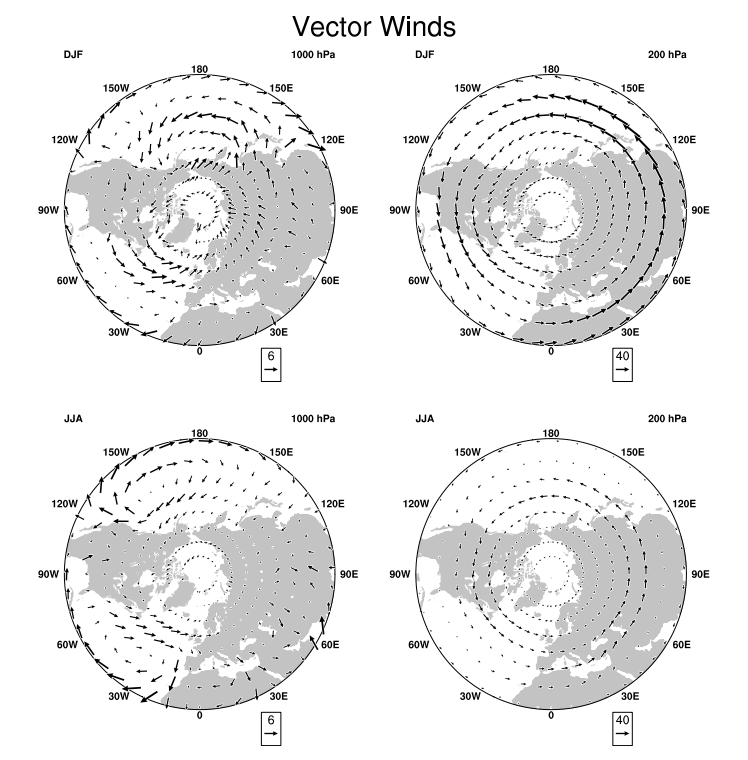
\includegraphics[width=\textwidth]{figures/vectorwinds.png}
            \caption{Figure and caption sourced from \cite{Hurrell2003}. Mean vector winds for (top) boreal winter (December-February) and (bottom) boreal summer (June-August) for (left) 1000~hPa and (right) 200~hPa over 1958-2001. The scaling vectors are indicated in the boxes and are given in units of m/s.}
            \label{fig:vectorwinds}
        \end{figure}
    
        \cite{ClimateReanalyzer2023} provides access to common environmental variables through reanalysis data from the ECMWF and NCEP, as well as indices and gridded observations from NOAA. In addition, they offer access to tools for the creation of custom plots. In addition to the appendix figures that confirm 1000hPa wind vectors, we include Figures \ref{fig:CR_10m_wind_DJF} and \ref{fig:CR_10m_wind_JJA}. These depict average 10m wind speed during boreal winter (DJF) and summer (JJA) from 1950 to 2020, aligning with the study's time frame. While these figures do not offer specific insights into windstorms or their relationship with the NAO, they should enhance the reader's grasp of Europe's environmental conditions and highlight areas prone to windy weather.
        
        \begin{figure}
            \centering
            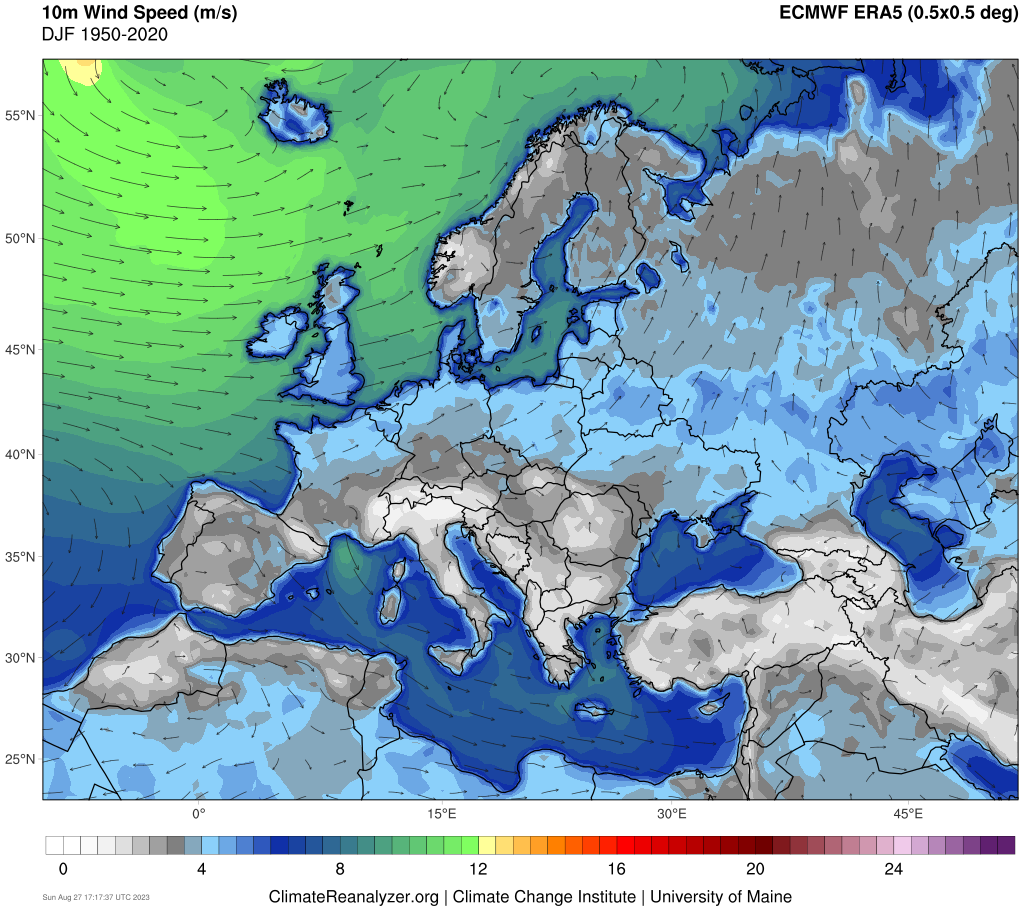
\includegraphics[width=\textwidth]{figures/era5-0p5deg_68.png}
            \caption{Sourced from \cite{ClimateReanalyzer2023}. 10m average Wind Speed in m/s for the December-January-February period over the years 1950 to 2020. Based on ECMWF ERA5 reanalysis data.}
            \label{fig:CR_10m_wind_DJF}
        \end{figure}
    
        \begin{figure}
            \centering
            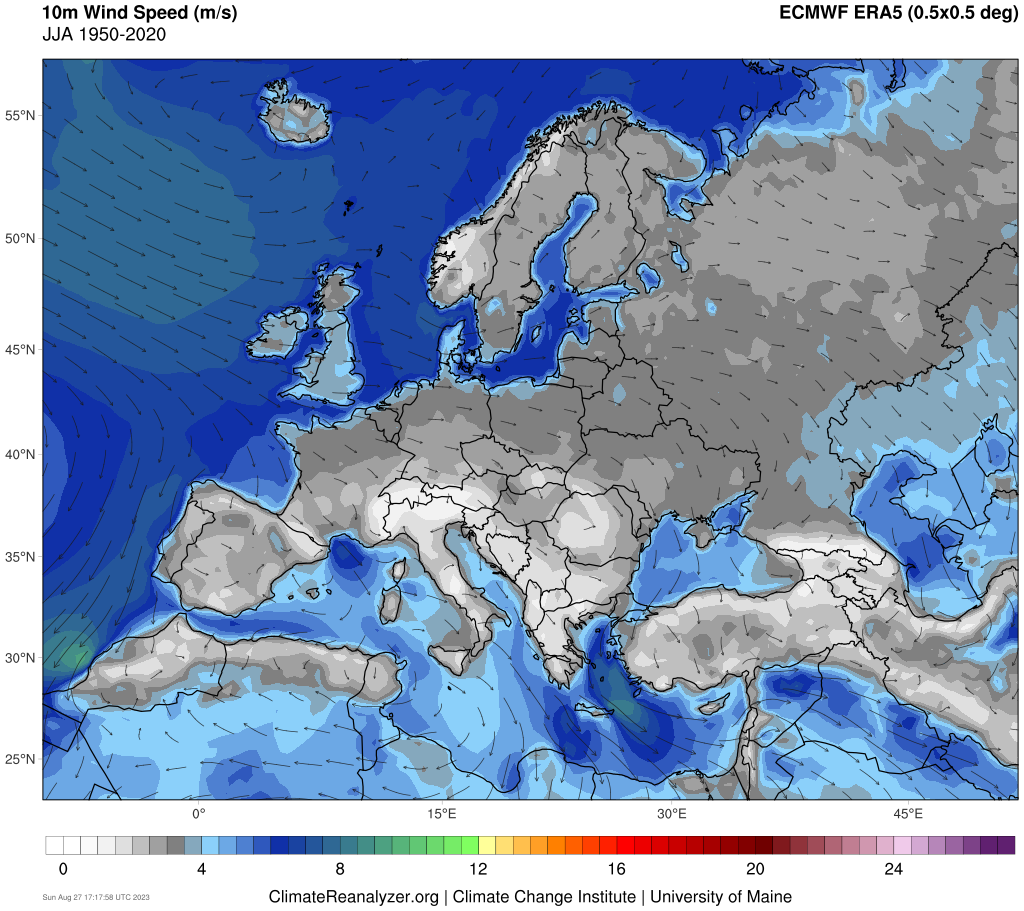
\includegraphics[width=\textwidth]{figures/era5-0p5deg_26.png}
            \caption{Sourced from \cite{ClimateReanalyzer2023}. 10m average Wind Speed in m/s for the June-July-August period over the years 1950 to 2020. Based on ECMWF ERA5 reanalysis data.}
            \label{fig:CR_10m_wind_JJA}
        \end{figure}
    
        \cite{https://doi.org/10.1002/joc.1982} and \cite{https://doi.org/10.1002/2014GL059647} observe, based on windstorm data between 1950 and 2010, that in addition to their findings aligning with those of \citeauthor{TheEffectsofNorthAtlanticSSTandSeaIceAnomaliesontheWinterCirculationinCCM3PartIMainFeaturesandStormTrackCharacteristicsoftheResponse} and \citeauthor{Hurrell2003}, windstorms are most likely to develop during moderately positive NAO phases. 
    
        In 2009, \cite{Pinto2009} published a significant statistical analysis of extreme cyclones and their relation to the NAO, as well as the variables that dominate their intesification: latent energy, upper-air baroclinicity, horizontal divergence, and jet stream strength. They explain the higher intensity of positive NAO cyclones to be due to the larger area with conditions that promote growth. \cite{HURRELL200928} similarly identify the NAO as important to the development and intensity of windstorms through its effect on the heat content of the Atlantic ocean.
    
        Using hindcasts from the 1$^{st}$ November, \cite{Renggli2011} finds a significant predictive skill for the frequency of December to February windstorms in the 1980–2001 period. Predictive skill in the 1980–2001 period is measured to be higher than that for the 1960–2001 period. Additionally, the level of skill turns out to be related to the frequency of storms in a given winter. Generally, winters with high storm frequency are better predicted than winters with medium storm frequency. Looking at their findings today, the author believes that this tendency might be due to the signal-to-noise ratio in models. Winters with high storm frequency will most likely have more ensemble members forecasting a windstorm in their simulation. As such the SNR will be higher as compared to low-windstorm frequency winters, where only few members will predict a windstorm and the forecast might be drowned out in the ensemble average.
    
        \cite{Scaifehttps://doi.org/10.1002/2014GL059637} reports on advances in modelling that allow the NAO to be predicted months in advance, this skill extending to winter storminess and wind speed. Furthermore, winter extremes are shown to be predictable, which allows for the forecasting of windstorms. \citeauthor{Scaifehttps://doi.org/10.1002/2014GL059637} use the Met Office Global Seasonal Forecast System 5 (GloSea5). They report that due to an anomalously low signal-to-noise ratio, a paradox emerging in climate models described in detail by \cite{Scaife2018}, large ensembles are needed to achieve a given level of skill. This work is expanded on by \cite{Scaife2016}, where stratospheric events such as sudden stratospheric warming (SSW) and strong polar vortex (SPV) are linked to a shift in the NAO. Similarly to \citeauthor{Scaifehttps://doi.org/10.1002/2014GL059637}, \cite{Palin2016} and \cite{Clark_2017} report on a statistically significant relationship between the NAO and hazardous weather conditions during winter in the UK, in particular of wind speed and wind power. 
    
        In 2018, for the first time, \cite{Befort2018} shows a significant ability to forecast the winter frequency of extratropical storms and high-impact windstorms associated with them, in areas prone to such events. This is an improvement over \cite{Renggli2011} as \citeauthor{Befort2018} produces a forecast, while the former report their predictive ability in hindcasts. Although the forecasts produced are statistically significant, the reported skill is still low to medium. Forecasts using the NAO as a predictor of windstorms are more successful over the British Isles and North Sea in MetOffice-GloSea5 and ECMWF-System4, but less so over central western Europe. The skill improves by combining this technique with the inclusion of an objective tracking algorithm.
    

    
    \subsection{Where we are today}

        The latest report, at the time of writing this work, is that of \cite{Degenhardt2023}. In it, two approaches to windstorm forecasting are compared by their ability to predict frequency of events during the winter season and the accumulated severity of windstorms for that season. The first method is referred to as a 'direct' method and consists of identifying and tracking storms in individual members of the seasonal hindcast ensembles in the MetOffice-GloSea5.
        The second method, named as 'indirect', is also used in \cite{Befort2018} and \cite{Scaifehttps://doi.org/10.1002/2014GL059637}. In it, storm parameters are calculated via a statistical regression, based on a combination of large-scale patterns as predictors (NAO, Scandinavian Pattern - SCA, and East-Atlantic Pattern - EA). \citeauthor{Degenhardt2023} builds a multiple linear regression model for each of the parameters they want to investigate.

        Both methods report skill similar to that of previous studies such as \cite{Befort2018} and \cite{Scaifehttps://doi.org/10.1002/2014GL059637} when the predicted parameter is the frequency of the storms. The statistical method used by \cite{Renggli2011} produces better results for winters with frequency of windstorms in the lower or upper tercile. The main difference between the direct and indirect methods is their ability to predict the severity parameter. The indirect method performs better when all predictor indices are incorporated - the NAO, SCA and EA in comparison to statistical regression methods that solely use the NAO. Despite this improvement, the indirect method is still second to the skill displayed by the direct method. In their work, \citeauthor{Degenhardt2023} report an anomalously low signal-to-noise ratio, as described in \cite{Scaife2018}, similarly to other previous studies.

        In an unpublished work, \cite{Priestley2023} explore a new statistical technique to obtain wind gusts throughout Europe using observed windstorm footprints. Through this method, high return period losses can be assessed without the complexities of a full catastrophe model.


\section{Existing SSI Methods}
    
    Having a quantitative measure of windstorm severity is important for both the private sector (research, (re)insurance) and the public sector (public safety, resource allocation). To achieve this measure, the concept of a Storm Severity Index is introduced. SSI's can be largely split into two categories: impact-based and meteorological. The former includes a measure of vulnerability, such as population or amount of infrastructure. An SSI using this measure will yield a higher index for windstorms over a town than over uninhabited areas. The latter method is concerned solely with the attributes of the storm and is a purer measure of severity. In this study, we use a meteorological method.

    \subsection{Description and Examples of Existing Methods}

        As defined in \cite{ADictionaryofWeather}, a Storm Severity Index is a measure of the severity of storms in the form of Equation \ref{eq:SSIDictionary}, where $\mathbf{V}$ is the maximum surface velocity of the wind, $\mathbf{A}$ is the largest surface area containing damaging winds and $\mathbf{D}$ is the duration of time.

        \begin{equation}
            \label{eq:SSIDictionary}
            \mathbf{V}^3 \cdot \mathbf{A} \cdot \mathbf{D}
        \end{equation}

        Of Equation \ref{eq:SSIDictionary} the one variable that remains the same in all variants of SSI is the component of the wind speed to the $3^{\text{rd}}$ power. The equation itself can be modified according to the needs of the study. An example is the SSI used by the Copernicus Extreme Windstorm Catalogue given in Equation \ref{eq:SSI_XWS}, where $\mathbf{V}_{\text{max}}$ is the maximum wind speed of the storm and $\mathbf{A}$ is the size of the storm over land for which the maximum gust exceeds 25mps. In this version of Equation \ref{eq:SSIDictionary}, the duration $\mathbf{D}$ does not appear, as this SSI is only concerned with the instant for which the storms wind is most violent. In this form of the SSI, \cite{XWS-nhess-14-2487-2014} find that the classification of windstorms best identifies those with high insurance loss.

        \begin{equation}
            \label{eq:SSI_XWS}
            \text{SSI}_{\text{XWS}} = \mathbf{V}_{\text{max}}^3 \cdot \mathbf{A}
        \end{equation}

        For another example, we can look at the SSI method used by a reinsurance company given in Equation \ref{eq:SSI_AON}. $\mathbf{V}_{\text{Filtered}}$ is given by Equation \ref{eq:SSI_AONDef} and $\mathbf{A}$ has a similar filter applied such that only the area where the winds exceed 20 meters per second is included in the sum. This method is more thorough than the XWS method as it breaks the storm into grids and considers the wind speed in each individual cell. It also uses a lower threshold and as such is more suitable when studying a broader range of storms, while the above is focused on identifying only the most severe of events.

        \begin{equation}
            \label{eq:SSI_AON}
            \text{SSI}_{\text{AON}} = \frac{\sum_{\text{Grids}}\left(\mathbf{V}_{\text{Filtered}}\right)^3 \cdot \mathbf{A}}{\mathbf{A}_{\text{Country}}}
        \end{equation}

        \begin{equation}
            \label{eq:SSI_AONDef}
            \mathbf{V}_{\text{Filtered}} = 
                \begin{cases}
                    \mathbf{V}_{\text{Wind}} - 20\left[m/s\right] & \mathbf{V}_{\text{Wind}} > 20 \\
                    0                                             & \text{otherwise} \\
                \end{cases}
        \end{equation}

% CHAPTER 3
\chapter{Data and Methodology}
    \section{Data Review}

    \subsection{NAO Data}

        Information about the state of the North Atlantic Oscillation, both daily and monthly, as used in this project, is available through the National Oceanic and Atmospheric Administration (NOAA) web portal. The calculation basis for the index is based on \cite{ClassificationSeasonalityandPersistenceofLowFrequencyAtmosphericCirculationPatterns}, employing Rotated Principal Component Analysis (RPCA) on monthly standardised 500-mb height anomalies from the CDAS within $20^\circ$N to $90^\circ$N from 1950 to 2000. The anomalies are determined by comparing the daily mean and standard deviation of the climatological average of 1950-2000 with the current values.
        
    \subsection{Storm Track Data}
    \label{sec:stormtrackdata}

        The foundation of this project are storm tracks provided by Hodges K. (2023). These tracks are primarily sourced from the European Centre for Medium-Range Weather Forecasts (ECMWF) reanalysis project, ERA5 \citep{ERA5globalreanalysishttps://doi.org/10.1002/qj.3803}. They were generated by a tracking algorithm designed to identify and follow points of relative vorticity at 850~hPa as outlined in \cite{NewPerspectivesontheNorthernHemisphereWinterStormTracks}, \cite{AdaptiveConstraintsforFeatureTracking}, and \cite{FeatureTrackingontheUnitSphere}. The tracks cover a period from 1940 to 2022 and have higher spatial resolution than tracks generated through older ERA projects, with the new tracks making use of T63 versus older projects based on T42, resulting in a decrease in grid cell spacing from roughly $2.8^\circ$ to $1.9^\circ$. The temporal resolution has also been increased from 3 to 1 hour.
        
        The tracks contain hourly data on the points of greatest relative vorticity, lowest mean sea-level air pressure, highest wind speed recorded around the storm at 925~hPa and highest wind speed recorded around the storm at 10m above the surface along with the relevant position in latitude and longitude for each of the listed data points.

        In this project, we also make use of the Extreme Wind Storms (XWS) catalogue \citep{XWS-nhess-14-2487-2014}. A publicly available catalogue containing information on European windstorms, covering 1979 to 2012, and consists of severe events that have caused high (re)insurance loss or have associated with them a high Storm Severity Index (SSI). SSI is calculated as a function of the storm area and maximum 925~hPa wind speed.
        
    \subsection{Wind Data}

        ERA5-Land, developed by \cite{munoz2019era5land} and the ECMWF, is an improvement on the ERA5 dataset and focuses exclusively on variables over land, spanning the period 1950 to 2023. It makes use of a finer grid spacing than ERA5, $0.1^\circ$ by $0.1^\circ$ ($\approx 9 \times 9 $km) compared to $0.25^\circ$ by $0.25^\circ$ ($\approx 23 \times 23 $km). The lapse rate has been adjusted to account for this higher spatial resolution and integrates ERA5 atmospheric variables as atmospheric forcing.

        ERA5-Land data are organised as follows: Each dataset comprises numerous data points distributed across a geographic grid. Consider each point as a representation of wind speed, orientated either North or East. These points are organised within a matrix, where rows and columns correspond to latitude and longitude, respectively. Thus, by identifying a point's position within the matrix, we can deduce its geographical coordinates. The dimensions of this matrix reflect our designated study area, and each matrix pertains to a specific moment, such as 14:00 on 01 Jan 1990. For every timestamp, two matrices are available: one for Northward wind measurements and another for Eastward ones. Together, these matrices allow us to determine both the magnitude and direction of the wind. These matrices are updated every hour, and the spacing between individual points in a matrix is 0.1 degrees.

\section{The New SSI Method}

    For the purposes of this study, a new method is developed to estimate the destructiveness of windstorms. It does this based on the energy carried by the wind near the surface, which is calculated by modifying the classic Kinetic Energy equation (Equation \ref{eq:KEfundamental}) and the equation for Mass Flow Rate (Equation \ref{eq:MassFlowRate}).
    
    \begin{equation}
    \label{eq:KEfundamental}
        \mathbf{KE} = \frac{1}{2} m\mathbf{v}^2
    \end{equation}

    \begin{equation}
    \label{eq:MassFlowRate}
        \dot{m} = \rho \mathbf{v} \cdot \mathbf{A}
    \end{equation}

    Where $\mathbf{KE}$ is the Kinetic Energy in the direction of the velocity vector, $m$ is the mass of the object, and $\mathbf{v}$ is the velocity vector taken to be the speed and direction of the wind at 10 m. $\dot{m}$ is the change in mass with respect to time of a fluid, $\rho$ is the density of the fluid and in this study is set to a constant value of $\rho = \rho_{air}\, \left(20^{\circ}C,\: 1024hPa\right) \approx 1.2$ kg/m$^3$. $\mathbf{A}$ is the cross-sectional vector area, with its surface orthogonal and its direction perpendicular to the velocity vector (Figure \ref{fig:volumeflowrate}). $\mathbf{A}$ has a fixed height of 10m, while its width is a function of wind direction, latitude, and longitude. The complete methodology for calculating $\mathbf{A}$ is presented in Section~\ref{sec:Calculating the cross-sectional vector area}. 

    \sidecaptionvpos{figure}{t}
    \begin{SCfigure}
        \centering
        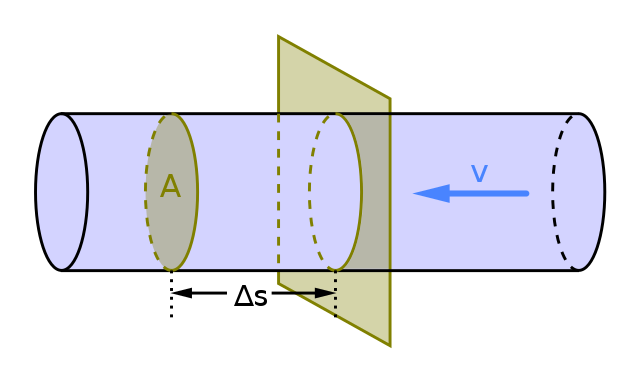
\includegraphics[width=0.6\textwidth]{figures/640px-Volumetric-flow-rate.svg.png}
        \caption{Visualisation of mass flow rate, with $\mathbf{v}$ the velocity vector and $\mathbf{A}$ the cross-sectional vector area. Adapted from MikeRun via Wikimedia Commons under license CC BY-SA 4.0. $\Delta \mathbf{s}$ is related to the volume flow rate and can be ignored.}
        \label{fig:volumeflowrate}
    \end{SCfigure}
    
    To combine Equation \ref{eq:KEfundamental} and Equation \ref{eq:MassFlowRate} we express the mass $m$ through the mass flow rate $\dot{m}$. The first step is to separate variables for the derivative $\mathrm{d}m/\mathrm{d}t$, and then integrate, which transforms Equation \ref{eq:MassFlowRateIntegrating} into Equation \ref{eq:MassFlowRateIntegrated}.
    
    \begin{equation}
    \label{eq:MassFlowRateIntegrating}
        \int \mathrm{d}m = \int \rho \mathbf{v} \cdot \mathbf{A} \mathrm{d}t
    \end{equation}

    \begin{equation}
    \label{eq:MassFlowRateIntegrated}
        m = \rho \mathbf{v} \cdot \mathbf{A} t
    \end{equation}

    By substituting Equation \ref{eq:MassFlowRateIntegrated} into Equation \ref{eq:KEfundamental} (referenced as Equation \ref{eq:KEandMassFlow}), we derive Equation \ref{eq:KE}. This gives us the Kinetic Energy, in Joules, of the wind at 10m.

    \begin{equation}
    \label{eq:KEandMassFlow}
        KE = \frac{1}{2} \left(\rho \mathbf{v} \cdot \mathbf{A} t \right) \mathbf{v}^2
    \end{equation}

    \begin{equation}
    \label{eq:KE}
        KE = \frac{1}{2} \rho \mathbf{v}^3 \cdot \mathbf{A} t
    \end{equation}

    Applying Equation \ref{eq:KE} to a data grid in an area of interest allows us to study the strength of a storm in its entirety or focus on a particular location. It also provides a robust way of ranking long-lasting storms of moderate intensity against short-lived and violent events.

    To the best knowledge of the author, this method appears novel within the field; however, there are examples \citep{web:psuWindEnergy} where the underlying equation is used in estimating the energy supplied to wind turbines by taking a derivative with respect to time of Equation \ref{eq:KE} which provides the wind power in watts.
    
    \subsection{Rationale for Development}

        The primary purpose of developing the energy method is the need for a method which recognises the irregular structure of a windstorm. Winds inside a windstorm can vary in speed depending on topography, pressure gradients, temperature differences, etc. which means that storms with similar parameters such as maximum vorticity or highest wind gust can vary in destructiveness. Another problem the energy method addresses is the difference between storms that are destructive not because of the severity of their winds, but because of their size and duration, where the loss accumulates and can become just as costly as a more violent event.

        It is of increased complexity compared to more common methods and requires the execution of code, including when obtaining an SSI for a singular storm/event. It is based off of wind data over the area of interest, and its performance is proportional to the resolution of the data, both in space and in time. 
        
\section{Analysis of Wind Energy in Storms}
    \subsection{Finding a Windstorm}

        The first step to analysing windstorms is knowing when and where a windstorm is. In this section, we go over the method used to sieve through storm track data (see Section \ref{sec:stormtrackdata} for more information on storm tracks) in order to compile a list of relevant windstorms and their start and end dates. The first step is to narrow the storm tracks to only those within our area of interest - western Europe, excluding Iceland ($\phi \in (42^\circ \rightarrow 72^\circ$\textbf{N}), $\lambda \in (-12^\circ \rightarrow 32^\circ$\textbf{E})).

        Since not all storm tracks develop into windstorms, we also apply a wind speed threshold that excludes data points that have a wind speed below 20~m/s at 10m. While there is not a consensus on the exact wind speed which defines a windstorm, we can estimate a range by observing past windstorm events and through the Beufort wind strength scale. Beufort 8 wind speeds, starting at 17~m/s, mark the point after which the wind becomes destructive to the environment. For Beufort 8, this manifests itself in the form of twigs and branches snapping off of trees. In this study, we will consider 17~m/s to be the minimum border for winds that can be considered part of a windstorm. The windstorm with the lowest maximum wind speed in the XWS Catalogue is windstorm Emma with 25~m/s at 925hPa over land. Thus 25~m/s is most likely the maximum threshold we can set without being overly exclusive. 20~m/s was selected through trial as the value within this range that best captures the storms listed in the XWS Catalogue.
        
        % As the track data were global and not limited to a particular location, a rough filter was applied, which excluded any data outside of a region of interest defined to be within 72 to 42 North and 12 West to 32 East. The resulting list of tracks contained noise in the form of tracks that did not develop into a storm. The reason for this is that when following a storm track, a point of low pressure and high vorticity is identified and followed over time, with wind speed measured in a fixed radius around the centre of the storm, but the method does not discriminate for the wind speed itself. To address this, another filter was added that removed all datapoints with wind speed below a certain threshold, in this study set at 20~m/s. This is a high threshold as windstorms are considered to be destructive at 17~m/s which coincides with the lower end of Beufort 8 winds, the point at which twigs begin to break off of trees, and slight structural damage can occur.
        
        Before further filtering was applied the result of implementing a minimum wind threshold resulted in a significant ammount of data points positioned over water, however, we are interested in windstorms over land as that is where they are most impactful. Due to the higher thermal conductivity of water and the lack of topographical obstacles, many storms in the dataset had their lifetime maximum over the water. Even storms that had a centre over land (determined by the point of highest vorticity) would continue displaying their wind speed over the ocean and as such it is challenging to estimate their destructiveness on land. To overcome this issue, we create a filter which removes all data points of storms with a centre above water and a wind speed below the threshold. The remaining fractions of storm tracks have a high potential of belonging to European windstorms. The reason we say that they are fractions of storm tracks is that as a storm centre moves on and off land, due to the removal of all points over water, gaps in the track appear. To fix this patch and to be able to measure windstorm impact before its centre is above our region of interest, for each data point, a 72-hour window was established, centred around the data point, comprising 36 hours both before and after the data point's timestamp. This process generated a series of "events", each spanning 72 hours. If any two events overlapped in time, they were consolidated into a single event. The start of this combined event was determined by the earlier of the two original events, and its end by the latter of the two.
        
        %Many of these storms would have their lifetime maximum wind be over the water which passed the wind speed criteria over water would quickly lose their energy once they moved onto land due to the lower heat capacity of the ground combined with the effects of topography. 
        
        %As the track data provided the highest recorded value of wind around a storm, the location of the highest wind would always be above water. Then, after reaching land, the storm loses energy over the colder ground, and the movement of air becomes impeded by increased friction and topographic characteristics. This meant that for storms that were only partially over land, the highest wind speed would be the one estimated over water, which introduced an inflated sense of the actual severity of a windstorm. As such, it became clear that storm tracks alone would be insufficient to complete the project, and tracks would serve better as a guide. 
        
        %If we apply a mask onto the stormtrack data and look at only storms whose centre was within the land contours of European countries, and increase the wind speed treshhold to 20~m/s we create a list containing the time at which storms touch ground. The first datapoint of each track is the time at which its point of highest vorticity is over land, and subsequent data points exist only as long as some part of the storm is over water, so that it can still meet the 20~m/s treshhold (a storm which is in its entirety over land very rarely meets these requirements). There were such cases where a storm would meet the criteria as it passes over the UK; this would allow data points to be saved, but a gap existed as it moved between the island and continetal Europe. To fix this patch and to be able to measure windstorm impact before its centre is above our region of interest, for each data point, a 72-hour window was established, centred around the data point, comprising 36 hours both before and after the data point's timestamp. This process generated a series of "events", each spanning 72 hours. If any two events overlapped in time, they were consolidated into a single event. The start of this combined event was determined by the earlier of the two original events and its end by the latter of the two.
        
        The resulting list of events becomes the guiding list of storms for the project. It was benchmarked by comparing the start time and end time of events within the list with those of named storms, as given by the XWS Extreme Wind Storm Catalogue. By manipulating the threshold for wind speed of storm track data, as well as the size of time window around each data point, we were able to fine-tune it to the values presented above, which performed the best. If the threshold was set lower, too many events would occur, and even with a shorter time window, many would overlap, creating windstorm events lasting unnaturally long and often merging two windstorms into one. Setting the treshold at 20~m/s and manipulating the window length, it was observed that for windows below 36 hours, events from our list would coincide roughly with 75\% of named storm events with an average of 2 or 3 additional days. This means that if a named storm were observed to start on 01/Jan to 10/Jan, what we might observe in our list would be an event starting 03/Jan to 13/Jan. With our chosen window of 36 hours before and after, we encapsulated on average 93\% of events with 4.2 additional days.

        Ultimately, for our methods, it is beneficial to make the trade of overestimating the timespan of an event, as when obtaining the energy of a windstorm, we only include data points with winds above 15~m/s. Therefore, additional days do not skew results as winds are unlikely to surpass such speeds before the start or after the end of a windstorm. This method struggles with separating multiple windstorm events when they are only a day or two apart.
        
        %CONTINUE HERE
        %List table, talk about the role of the threshold in the era5land data which means that we prefer events that cover a higher percent of storm events despite the cost of extra days, since they get filtered out due to their low wind speeds.
        
            

    \subsection{Calculating the cross-sectional vector area $\mathbf{A}$}
    \label{sec:Calculating the cross-sectional vector area}

        The cross-sectional vector area $\mathbf{A}$ is a rectangle with a height and a width, one can imagine it as a screen through which the wind passes through, with its value equal to its surface area and its direction orientated away and perpendicular to its face. In Figure \ref{fig:volumeflowrate} the area of $\mathbf{A}$ is normal to the flow of $\mathbf{v}$ and its direction is aligned with that of $\mathbf{v}$, so the dot product of the two vectors will simply be the multiple of the two numbers. In other words, the flow rate is greatest when the flow is directly against the screen. The height of $\mathbf{A}$ is 10~$m$ and its width is the distance of the diagonal inside a spherical quadrilateral, $0.1^\circ$ by $0.1^\circ$ in size, normal to the direction of the wind given by $\mathbf{v}$.

        Below we will explore how finding the length of this diagonal in meters is achieved. The equations below are a translation of the computational method, and there are some steps which the reader might believe are not in their simplest mathematical form. This is because they are not, with the trade-off being that for an increase in mathematical complexity we avoid \textsc{if} logical statements within the code, which increases efficiency and is a good coding practise, alltogether. The first step is to find the angle of the wind $\theta_{\mathbf{v}} = f(u = u_{\mathbf{v}},\: v = v_{\mathbf{v}})$ (Equation \ref{eq:theta}), where $u_{\mathbf{v}}$ is the Easterly component of the wind vector $\mathbf{v}$, and $v_{\mathbf{v}}$ is the Northerly component. We define a unit circle in the range $\left[ -180,\, 180 \right]$ such as the one presented in Figure \ref{fig:unitcircle}. Equation \ref{eq:theta} measures the angle between the x-axis and a line defined between the centre of the unit circle and a point with coordinates $P(x,y)=\left[u,\, v \right]$.

        \begin{SCfigure}
            \centering
            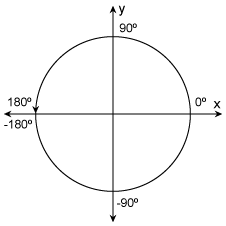
\includegraphics[width=0.4\textwidth]{figures/atan2d_graphic.png}
            \caption{Unit circle ranging from $-180^\circ$ to $180^\circ$, where the \textsc{x}-axis alligns with the East direction, and the \textsc{y}-axis alligns with North.}
            \label{fig:unitcircle}
        \end{SCfigure}
        
        \begin{equation}
        \label{eq:theta}
            \theta_{\mathbf{v}}(u, v) = 
            \begin{cases} 
                \text{tan}^{-1}\left(v/u\right)         & \text{if } u > 0 \\
                \text{tan}^{-1}\left(v/u\right)  + 180  & \text{if } v \geq 0 \; \wedge \; u < 0 \\
                \text{tan}^{-1}\left(v/u\right)  - 180  & \text{if } v < 0 \; \wedge \; u < 0 \\
                90                                              & \text{if } v > 0 \; \wedge \; u = 0 \\
                -90                                             & \text{if } v < 0 \; \wedge \; u = 0 \\
                \text{undefined}                                & \text{if } v = 0 \; \wedge \; u = 0
            \end{cases} 
        \end{equation}

        Knowing the angle of the wind vector $\theta_{\mathbf{v}}$, we can easily obtain the angle of the area vector $\theta_{\mathbf{A}}$ by rotating $\theta_{\mathbf{v}}$ by $90^\circ$ (Equation \ref{eq:thetaVtothetaA}). 

        \begin{equation}
        \label{eq:thetaVtothetaA}
            \theta_{\mathbf{A}}(\theta_{\mathbf{v}}) = \theta_{\mathbf{v}} + 90
        \end{equation}

        At this point, we have three pieces of information: the longitude $\lambda_P$ and latitude $\phi_P$ of the point at the centre of the grid cell, the size of the grid cell, and the fact that a line crosses the cell with an angle $\theta_{\mathbf{A}}$. If we can find the set of coordinates ($\left[\lambda_1,\, \phi_1\right]$, $\left[\lambda_2,\, \phi_2\right]$)  of the two points ($\mathbf{1}$, $\mathbf{2}$) that define this line, we can use the Haversine formula (Equation \ref{eq:haversine}), where $\Delta \phi = |\phi_1 - \phi_2|$, $\Delta \lambda = |\lambda_1 - \lambda_2|$ and $R$ is the radius of the earth $R = 6371$~km. The function $\mathbf{atan2}$ is defined as Equation \ref{eq:theta}.

        \begin{equation}
            \label{eq:haversine}
            \begin{aligned}
                a &= \text{sin}^2 (\Delta \phi / 2) + \text{cos}(\phi_1) \cdot \text{cos}(\phi_2) \cdot\text{sin}^2(\Delta \lambda /2) \\
                c &= \text{atan2}\left( \sqrt{a},\, \sqrt{1-a}\right) \\
                d &= R \cdot c
            \end{aligned}
        \end{equation}

        Given the conditions:
        
        \begin{equation}
            \begin{cases} 
                \text{TRUE} & (|\theta_{\mathbf{A}}| \leq 45) \vee \left(| \theta_{\mathbf{A}}| \geq 135 \right) \\
                \text{FALSE} & \text{else}
            \end{cases}
        \end{equation}
        
        We can define the transformations:
        
        \begin{equation} \label{eq:theta_transform}
            \theta' =
            \begin{cases} 
                90 - \left| \left(\theta_{\mathbf{A}} + 90\right) \bmod 360 - 180 \right| & \text{if } \text{TRUE} \\
                45 - \left| \left( \left|\theta_{\mathbf{A}}\right| + 90\right) \bmod 270 - 135 \right| & \text{else}
            \end{cases}
        \end{equation}
       
        Equation \ref{eq:theta_transform} defines transformations for $\theta' = f(\theta_{\mathbf{A}})$ such that the value of $\theta'$ is always between 0 and 45 as that is the range where $\text{tan}(\theta') \in (0,\, 1)$. The transformation functions ensure that when we calculate the coordinates for points $\mathbf{1}$ and $\mathbf{2}$  in Equations \ref{eq:lon1_transform} through \ref{eq:lat2_transform}, none fall outside the grid cell.
        
        \begin{equation} \label{eq:lon1_transform}
            \lambda_1 =
            \begin{cases} 
                \lambda_P + 0.05 \cdot
                    \begin{cases}
                        1  & \text{if } u \geq 0 \\
                        -1 & \text{else}
                    \end{cases}
                & \text{if } \text{TRUE} \\
                \lambda_P + 0.05 \cdot \tan(\theta') & \text{else}
            \end{cases}
        \end{equation}
        
        
        \begin{equation} \label{eq:lat1_transform}
            \phi_1 =
            \begin{cases} 
            \phi_P + 0.05 \cdot \tan(\theta') & \text{if } \text{TRUE} \\
            \phi_P + 0.05\cdot
                    \begin{cases}
                        1  & \text{if } v \geq 0 \\
                        -1 & \text{else}
                    \end{cases}
                & \text{else}
            \end{cases}
        \end{equation}
        
        
        \begin{equation} \label{eq:lon2_transform}
            \lambda_2 =
            \begin{cases} 
                \lambda_P - 0.05\cdot
                    \begin{cases}
                        1  & \text{if } u \geq 0 \\
                        -1 & \text{else}
                    \end{cases}
                    & \text{if } \text{TRUE} \\
                \lambda_P - 0.05 \cdot \tan(\theta') & \text{else}
            \end{cases}
        \end{equation}
        
        
        \begin{equation} \label{eq:lat2_transform}
            \phi_2 =
            \begin{cases} 
                \phi_P - 0.05 \cdot \tan(\theta') & \text{if } \text{TRUE} \\
                \phi_P - 0.05\cdot
                    \begin{cases}
                        1  & \text{if } v \geq 0 \\
                        -1 & \text{else}
                    \end{cases}
                    & \text{else}
            \end{cases}
        \end{equation}

        Following these steps and inserting the coordinates $\mathbf{1}\left[\lambda_1,\, \phi_1\right]$ and $\mathbf{2}\left[\lambda_2,\, \phi_2\right]$, into the Haversine set of equations given in Equation \ref{eq:haversine}, results in the length in metres of the cross-section vector area $\mathbf{A}$. This method makes the assumption that the Earth is perfectly spherical. The Earth's equitorial radius (6356~km) is 23~km larger than its polar radius (6378~km). This results in a maximum error of 0.5\% and is considered negligible for the distances measured for this project.
        
    \subsection{Obtaining Wind Energy}

        The energy of the windstorm is defined as the sum of the energy of the points in the area of interest for the duration of the windstorm event. The area of interest is every point within the following list of countries that is also within the boundary $\phi \in (42^\circ \rightarrow 72^\circ$\textbf{N}) and $\lambda \in (-12^\circ \rightarrow 32^\circ$\textbf{E}):

        Austria, Belgium, Czechia, Denmark, Estonia, Finland, France, Germany, Hungary, Ireland, Latvia, Liechtenstein, Lithuania, Luxemburg, the Netherlands, Norway, Poland, Slovakia, Spain, Sweden, Switzerland, and the UK.

        As we only count the energy of winds at or above 15~m/s, we do not need to know the exact borders of the windstorm, as the winds outside its area are unlikely to surpass that speed. A points energy can be calculated using Equation \ref{eq:KE}, with wind speed $\mathbf{v} = \sqrt{u^2_{\mathbf{v}} + v^2_{\mathbf{v}}}$, and the duration $t$ for which the equation is solved is $t = 1\text{hr}=3600\text{s}$. By changing the size of the list of countries which are counted towards the total energy of a windstorm, we can obtain the energy experienced during a windstorm event in a particular region or even a single country. This is useful for studying the severity of windstorms in different parts of Europe and for identifying zones particularly vulnerable to severe winds.
        
    \subsection{Challenges and Inaccuracies}

        Although the accuracy of the method depends on the spatial and temporal resolution of the reanalysis data used to calculate windstorm energies, its primary limitation arises from the storm "finding" technique. Specifically, the method sometimes struggles to pinpoint the precise start and end times of a storm. For certain storms, the 36-hour window before being recognised on land is insufficient. This is especially the case when the storm's centre moves parallel to the coast, likely tracing the path of a meridional jet stream. Consequently, the storm can accumulate significant damage to the infrastructure before the algorithm acknowledges it as an event. An example of this behaviour is the Great Storm of 87. 
        
        Another source of inaccuracy is the inability of the algorithm to distinguish between windstorm events that are only 2 to 3 days apart. In such a scenario, these storms are likely to be joined into a singular event, which may create outliers in the final results.

% CHAPTER 4
\chapter{Results: Performance of SSI methods}
    \section{Highlighting Named Storms}

    To estimate the ability of the algorithm to accurately capture the length of a windstorm, we experiment by appending different lengths of time to the points identified as belonging to a storm over land and with wind speed above 20m/s, as discussed in Chapter 3.3.1. The results of these experiments are presented in Table \ref{tab:stormcat}, where the second column contains the number of hours appended before/after the point in the format X/Y. We also identify the period during which the five cyclones produce windstorms over land, which does not always match the defined start and end time of the storm. This is achieved through the Copernicus Extreme Winds Catalogue, which provides animations representing the movement of cyclones and the strength of winds in western Europe, as well as information on the start and end dates of the storms. We chose 4 named storms and 1 severe but unnamed one: the Great Storm of '87, Lothar, Kyrill, Emma and a storm on the 13th of January 1993. All of the above storms have caused considerable damage and high insurance loss. 

        \begin{table}
        \centering
        \resizebox{0.95\textwidth}{!}{%
        \begin{tabular}{llllll}
        Windstorm   &       & Start       & End         & Match & Extra Days \\ \hline
        Emma        & data  & 25 Feb 2008 & 05 Mar 2008 &       &            \\
                    & DWOL  & 28 Feb 2008 & 5 Mar 2008  &       &            \\
                    & 24/12 & 29 Feb      & 04 Mar      & 75\%  & 0          \\
                    & 24/24 & 29 Feb      & 07 Mar      & 75\%  & 2          \\
                    & 30/24 & 29 Feb      & 07 Mar      & 75\%  & 2          \\
                    & 30/30 & 29 Feb      & 08 Mar      & 75\%  & 3          \\
                    & 36/36 & 20 Feb      & 08 Mar      & 100\% & 6          \\ \hline
        13 Jan '93  & data  & 12 Jan 1993 & 16 Jan 1993 &       &            \\
                    & DWOL  & 12 Jan 1993 & 16 Jan 1993 &       &            \\
                    & 24/12 & 08 Jan      & 15 Jan      & 80\%  & 4          \\
                    & 24/24 & 08 Jan      & 15 Jan      & 80\%  & 4          \\
                    & 30/24 & 07 Jan      & 15 Jan      & 80\%  & 5          \\
                    & 30/30 & 07 Jan      & 15 Jan      & 80\%  & 5          \\
                    & 36/36 & 07 Jan      & 16 Jan      & 99\%  & 5          \\ \hline
        G.S. of '87 & data  & 14 Oct 1987 & 19 Oct 1987 &       &            \\
                    & DWOL  & 14 Oct 1987 & 19 Oct 1987 &       &            \\
                    & 24/12 & 13 Oct      & 16 Oct      & 50\%  & 0          \\
                    & 24/24 & 13 Oct      & 17 Oct      & 66\%  & 0          \\
                    & 30/24 & 13 Oct      & 17 Oct      & 66\%  & 0          \\
                    & 30/30 & 13 Oct      & 17 Oct      & 66\%  & 0          \\
                    & 36/36 & 13 Oct      & 17 Oct      & 67\%  & 0          \\ \hline
        Lothar      & data  & 23 Dec 1999 & 28 Dec 1999 &       &            \\
                    & DWOL  & 22 Dec 1999 & 29 Dec 1999 &       &            \\
                    & 24/12 & 22 Dec      & 28 Dec      & 88\%  & 0          \\
                    & 24/24 & 22 Dec      & 29 Dec      & 99\%  & 0          \\
                    & 30/24 & 21 Dec      & 29 Dec      & 100\% & 1          \\
                    & 30/30 & 21 Dec      & 29 Dec      & 100\% & 1          \\
                    & 36/36 & 21 Dec      & 29 Dec      & 100\% & 1          \\ \hline
        Kyrill      & data  & 16 Jan 2007 & 21 Jan 2007 &       &            \\
                    & DWOL  & 16 Jan 2007 & 21 Jan 2007 &       &            \\
                    & 24/12 & 17 Jan      & 19 Jan      & 50\%  & 0          \\
                    & 24/24 & 17 Jan      & 22 Jan      & 83\%  & 0          \\
                    & 30/24 & 17 Jan      & 22 Jan      & 83\%  & 0          \\
                    & 30/30 & 17 Jan      & 22 Jan      & 83\%  & 1          \\
                    & 36/36 & 08 Jan      & 25 Jan      & 100\% & 10        
        \end{tabular}%
        }
        \caption{The ability of the algorithm to encompass a windstorm event. The numbers in X/Y format in the second column represent the amount of hours appended before/after a point identified as belonging to a storm over land and of wind speed above 20m/s. Storm data extracted from the Copernicus Extreme Winds Catalogue. DWOL represents the Days a Windstorm is Over Land.}
        \label{tab:stormcat}
        \end{table}

    As the appended number of hours increases, we observe an improved match between the dates during which windstorms occur for an event and the dates computed by the algorithm for the event. However, we also experience a growing number of noisy days, which are days outside the range of a storm. In this study, we make use of the fifth option which appends 36 hours on both ends of datapoints and minimise the noise from additional days by implementing a secondary wind speed threshold of 15m/s, the aim of which is to filter out any nonviolent winds. This way, we hope to filter out additional days as they will most likely not pass this test. However, this introduces the risk of merging two separate storms into a singular event if they occur with little time inbetween.

\section{Estimating Loss}

    We evaluated the ability of the storm energy-based SSI, developed for this study, to estimate insurance loss and found that it shows low correlation with a list of 50 storms extracted from the Copernicus Extreme Windstorm Catalogue. It performs similarly to another meteorologically focused SSI used in industry and presented in detail in Chapter 2. The energy-based SSI has a p-value of 0.60, while the one used in industry has a slightly higher p-value of 0.66. The reason for the poor performance in estimating loss is that both methods do not consider variables describing the vulnerability to damage in the area over which computation is performed, such as population or an infrastructural development index. We present a scatter plot in Figure \ref{fig:scatterSSI} illustrating the performance of both indices. Both models severely underestimated the loss caused by the Great Storm of '87, which moves along the western coast of Europe, but by the time it passes over land and is detected by the algorithms, it has already caused considerable damage.
    
        \begin{figure}
            \centering
            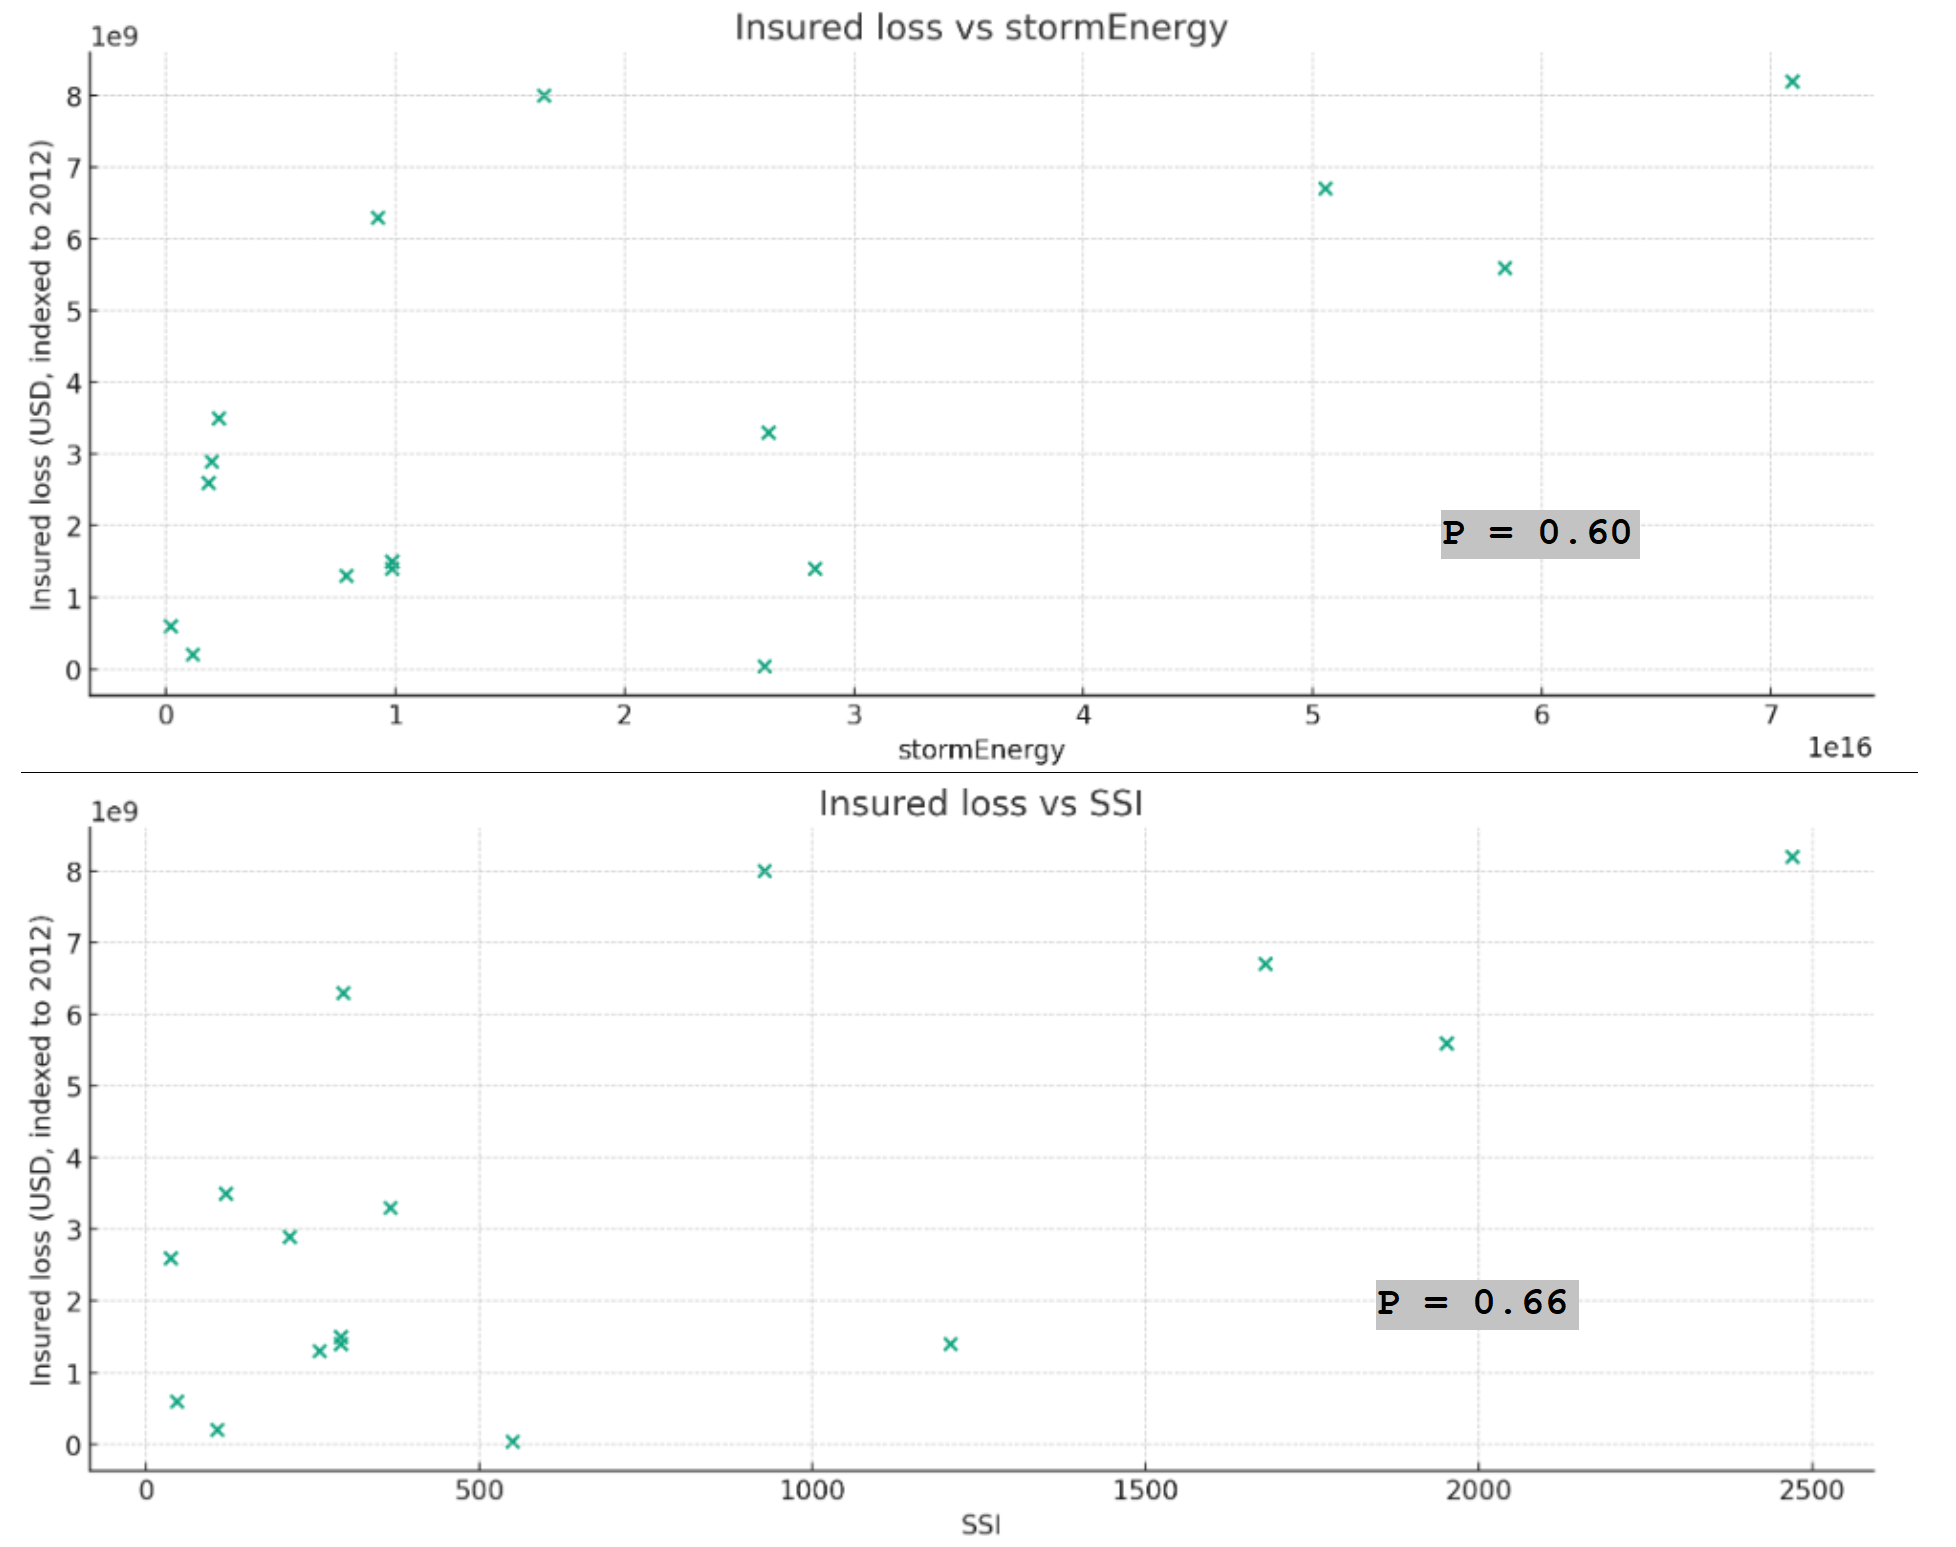
\includegraphics[width=\textwidth]{figures/ssiperformance.png}
            \caption{Performance of the storm energy based SSI method (above) versus an SSI used in industry (below). Both SSI are compared to insurance loss data provided by the Copernicus Extreme Windstorm Catalogue. The P value is reported as 0.60 for the energy method and 0.66 for the industry SSI.}
            \label{fig:scatterSSI}
        \end{figure}

    When estimating the effectiveness of various Storm Severity indices, particularly when they are not designed to measure damage to infrastructure, it is difficult to obtain a confident answer as to which one performs best for a specific measure. In further developing the storm-based SSI, the author hopes to create a detailed and reliable measure which considers all variables of a windstorm and can then be used to benchmark the performance of simpler and less computationally heavy SSIs.

% CHAPTER 5
\chapter{Results: EUWS and the NAO}
    In this chapter, we will not be discussing the results, but rather present them. This discussion will take place in Chapter 6. The results are grouped into three sections that correspond to the three main questions asked in this study. Before presenting them, we impel the reader to view Figures \ref{fig:naopostitivemap}, \ref{fig:naoneutralmapo} and \ref{fig:naonegativemapenter-label}. In addition to information about windstorm energy during different NAO phases, they illustrate the arrangement of the data points used to prepare the rest of the study. It is notable that all datapoints are positioned along the shoreline. This is an indicator that in the ERA5-Land reanalysis data, during a windstorm event, no points over the mainland exceed an hourly wind speed of 20m/s. The uncertainty introduced by this and what steps can be taken to mitigate this issue are discussed in Chapter 6.

The figures themselves are representative of all windstorms in the dataset and are divided into categories corresponding to the NAO index associated with the start of the event: NAO positive ($0.5 < \text{NAO}$), NAO neutral ($-0.5 \leq \text{NAO} \leq 0.5$) and NAO negative ($\text{NAO} < -0.5$). Figure \ref{fig:naopostitivemap} which corresponds to positive NAO events, shows considerably higher energies. Less apparent when comparing the figures with each other is the trajectory of windstorms during each NAO state. Regardless of the NAO state, high energy is always concentrated around the UK coastline; however, for NAO(+) events, energies are concentrated going North-East toward the Nordic countries through Denmark. NAO(0) events draw a trajectory that also passes through Denmark but is in the direction of Lithuania, Latvia, and Estonia. NAO(-) events take the southernmost trajectory passing through the Netherlands, Germany, Poland and towards the Ukraine. The author found that this trend can be seen most clearly when the three figures are saved and quickly flicked through back and forth to simulate a moving image. 

    \begin{figure}
        \centering
        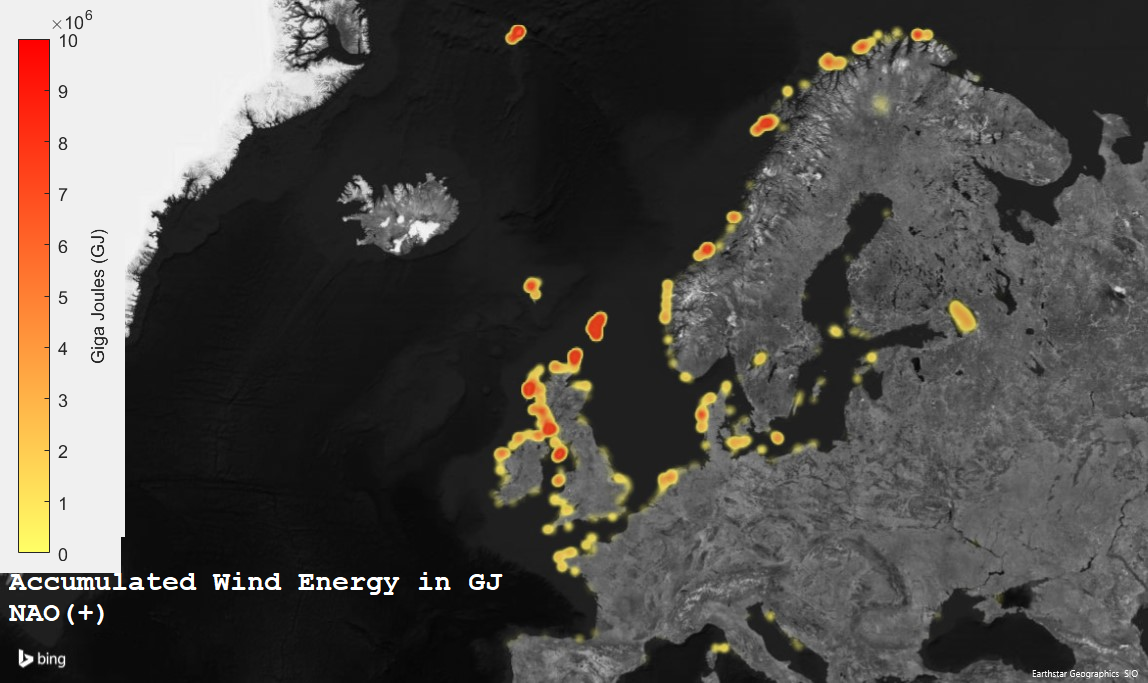
\includegraphics[width=\textwidth]{figures/NAOPOsitive.png}
        \caption{Heatmap of Energy accumulated from windstorms during NAO(+).}
        \label{fig:naopostitivemap}
    \end{figure}

    \begin{figure}
        \centering
        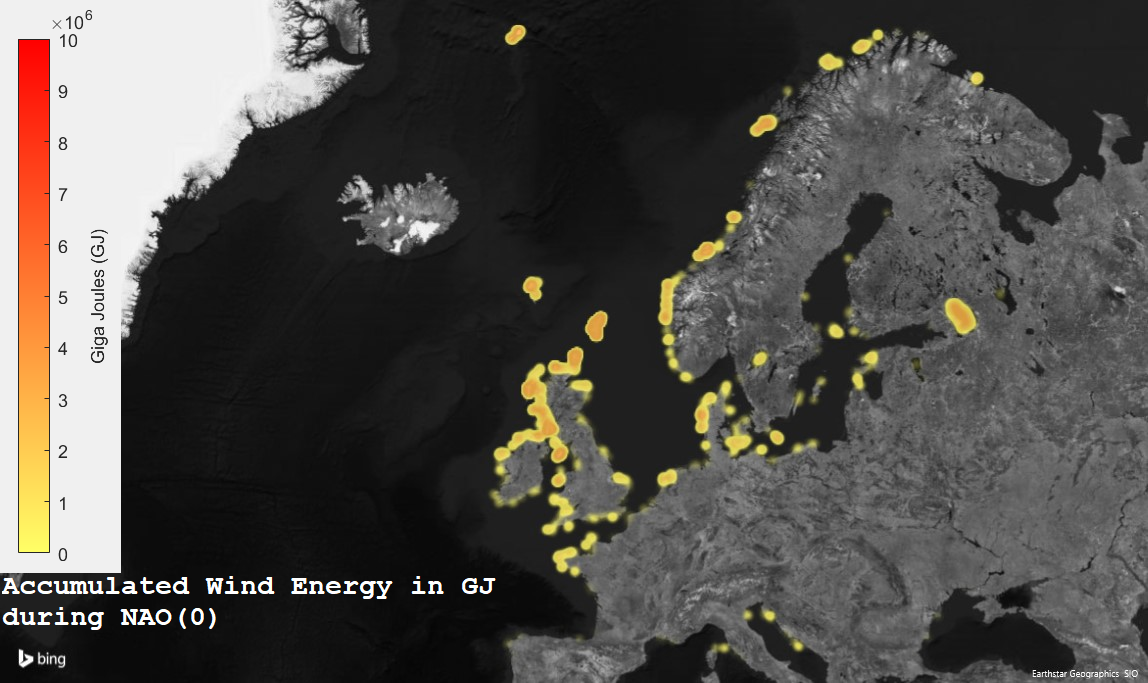
\includegraphics[width=\textwidth]{figures/NAONeutral.png}
        \caption{Heatmap of Energy accumulated from windstorms during NAO(0).}
        \label{fig:naoneutralmapo}
    \end{figure}

    \begin{figure}
        \centering
        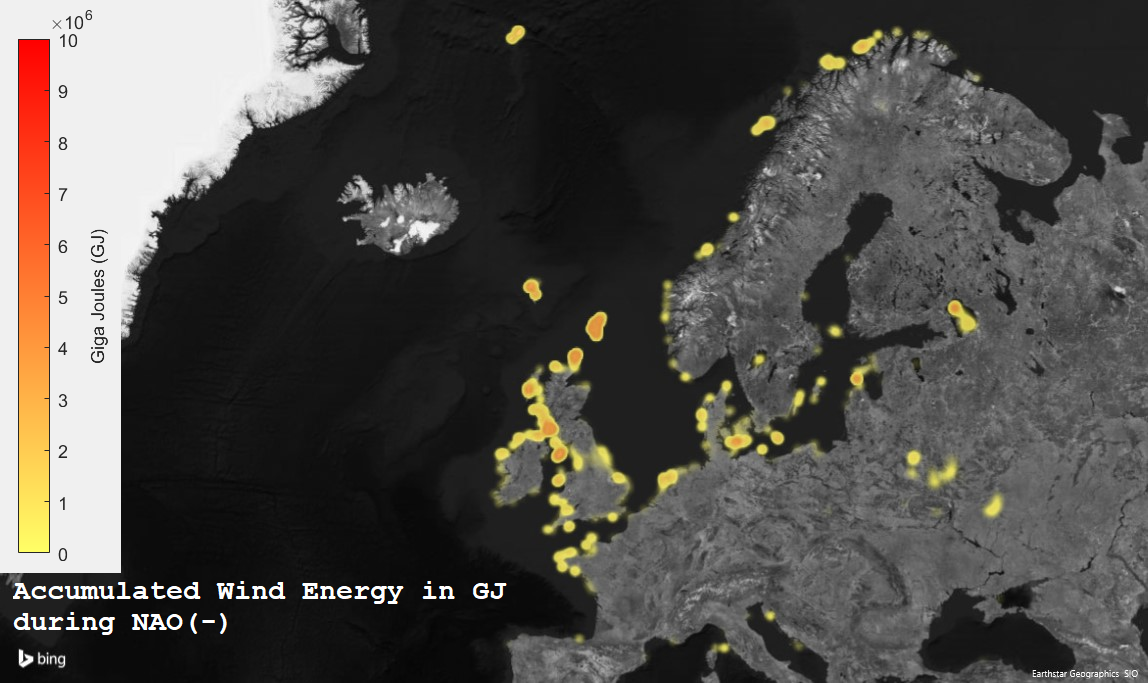
\includegraphics[width=\textwidth]{figures/NAONegative.png}
        \caption{Heatmap of Energy accumulated from windstorms during NAO(-).}
        \label{fig:naonegativemapenter-label}
    \end{figure}



\FloatBarrier
\section{Risk of European Windstorm during NAO Neutral Index}

    To estimate the return period of European Windstorms for neutral NAO phases, we will look at the statistical distribution of events and their associated indices. We begin with Figures \ref{fig:storm_count_vs_daily_nao} and \ref{fig:storm_count_vs_monthly_nao}. The former represents daily NAO values, while the latter uses monthly, where the NAO index of a windstorm is that of the first day of the event. In both cases we can see that the maximum number of events occur when the NAO is slightly positive, which agrees with the findings of \cite{https://doi.org/10.1002/joc.1982} and \cite{https://doi.org/10.1002/2014GL059647}. 

        % FIGURE 1 ------------------------------------------------------------------------------------------------------------------------
        \begin{figure}[ht]
            \begin{minipage}[t]{0.6\textwidth}
                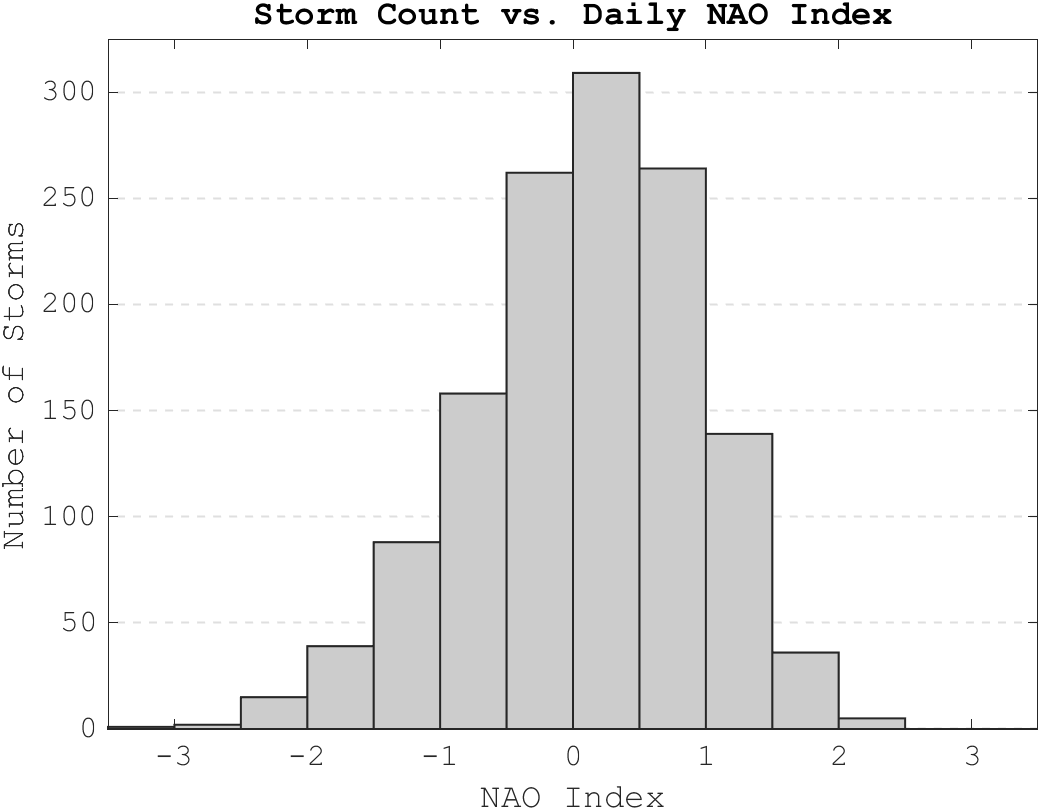
\includegraphics[width=\textwidth]{figures/Storm Count vs. Daily NAO.png}
                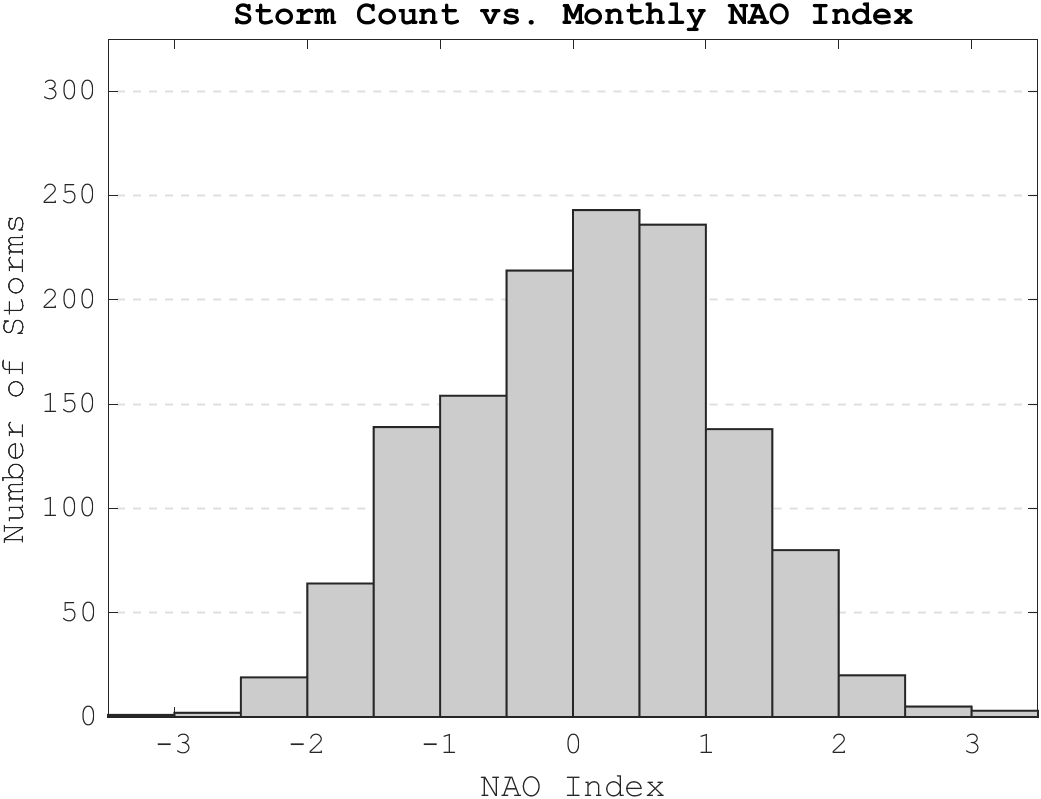
\includegraphics[width=\textwidth]{figures/Storm Count vs. Monthly NAO.png}
            \end{minipage}
            \hfill  % Fill horizontal space
            \begin{minipage}[t]{0.4\textwidth}
                \vspace*{-215pt}  % Move the start of the caption upwards. You might need to adjust this value.
                \caption{Storm Count vs. Daily NAO index from 1950 to 2020. For this figure, the NAO index of a storm is the index on the day the storm begins. The beginning of a storm in this study is defined as 36 hours before the centre (point of highest relative vorticity) of the storm touches land. N=1286.}
                \label{fig:storm_count_vs_daily_nao}
                \vspace*{88pt}  % Increase space between captions. You might need to adjust this value.
                \caption{Storm Count vs. Monthly NAO index from 1950 to 2020. Analogous to Figure \ref{fig:storm_count_vs_daily_nao}. N=1286.}
                \label{fig:storm_count_vs_monthly_nao}
            \end{minipage}
        \end{figure}
        %----------------------------------------------------------------------------------------------------------------------------------

    We follow up with an analysis of the distributing of NAO state over time. As in the last figure, we do this for both daily and monthly values in order to minimise any skewing of the data originating from inaccurately timing the start of a windstorm event. This distribution can be seen in Figure \ref{fig:nao_and_event_rate}A and Figure \ref{fig:nao_and_event_rate}C for daily and monthly values, respectively. Figures \ref{fig:nao_and_event_rate}B and \ref{fig:nao_and_event_rate}D are effectively the result of dividing the data in Figure \ref{fig:storm_count_vs_daily_nao} by that of Figure \ref{fig:nao_and_event_rate}A, and that of Figure \ref{fig:storm_count_vs_monthly_nao} by that of Figure \ref{fig:nao_and_event_rate} C, respectively, to obtain the monthly version of the spread. In \ref{fig:nao_and_event_rate}A and \ref{fig:nao_and_event_rate}C, we can see that the most probable state is when the NAO is slightly positive. In \ref{fig:nao_and_event_rate}B and \ref{fig:nao_and_event_rate}D, the probability of a windstorm occurring is uniform across all NAO states with an exception for the far ends of the data range. The author hypothesises that this is due to the very low sample size (N $<$ 5) in that range.
    
        % FIGURE 2 + FIGURE 3 -------------------------------------------------------------------------------------------------------------
        \begin{figure}
            \centering
            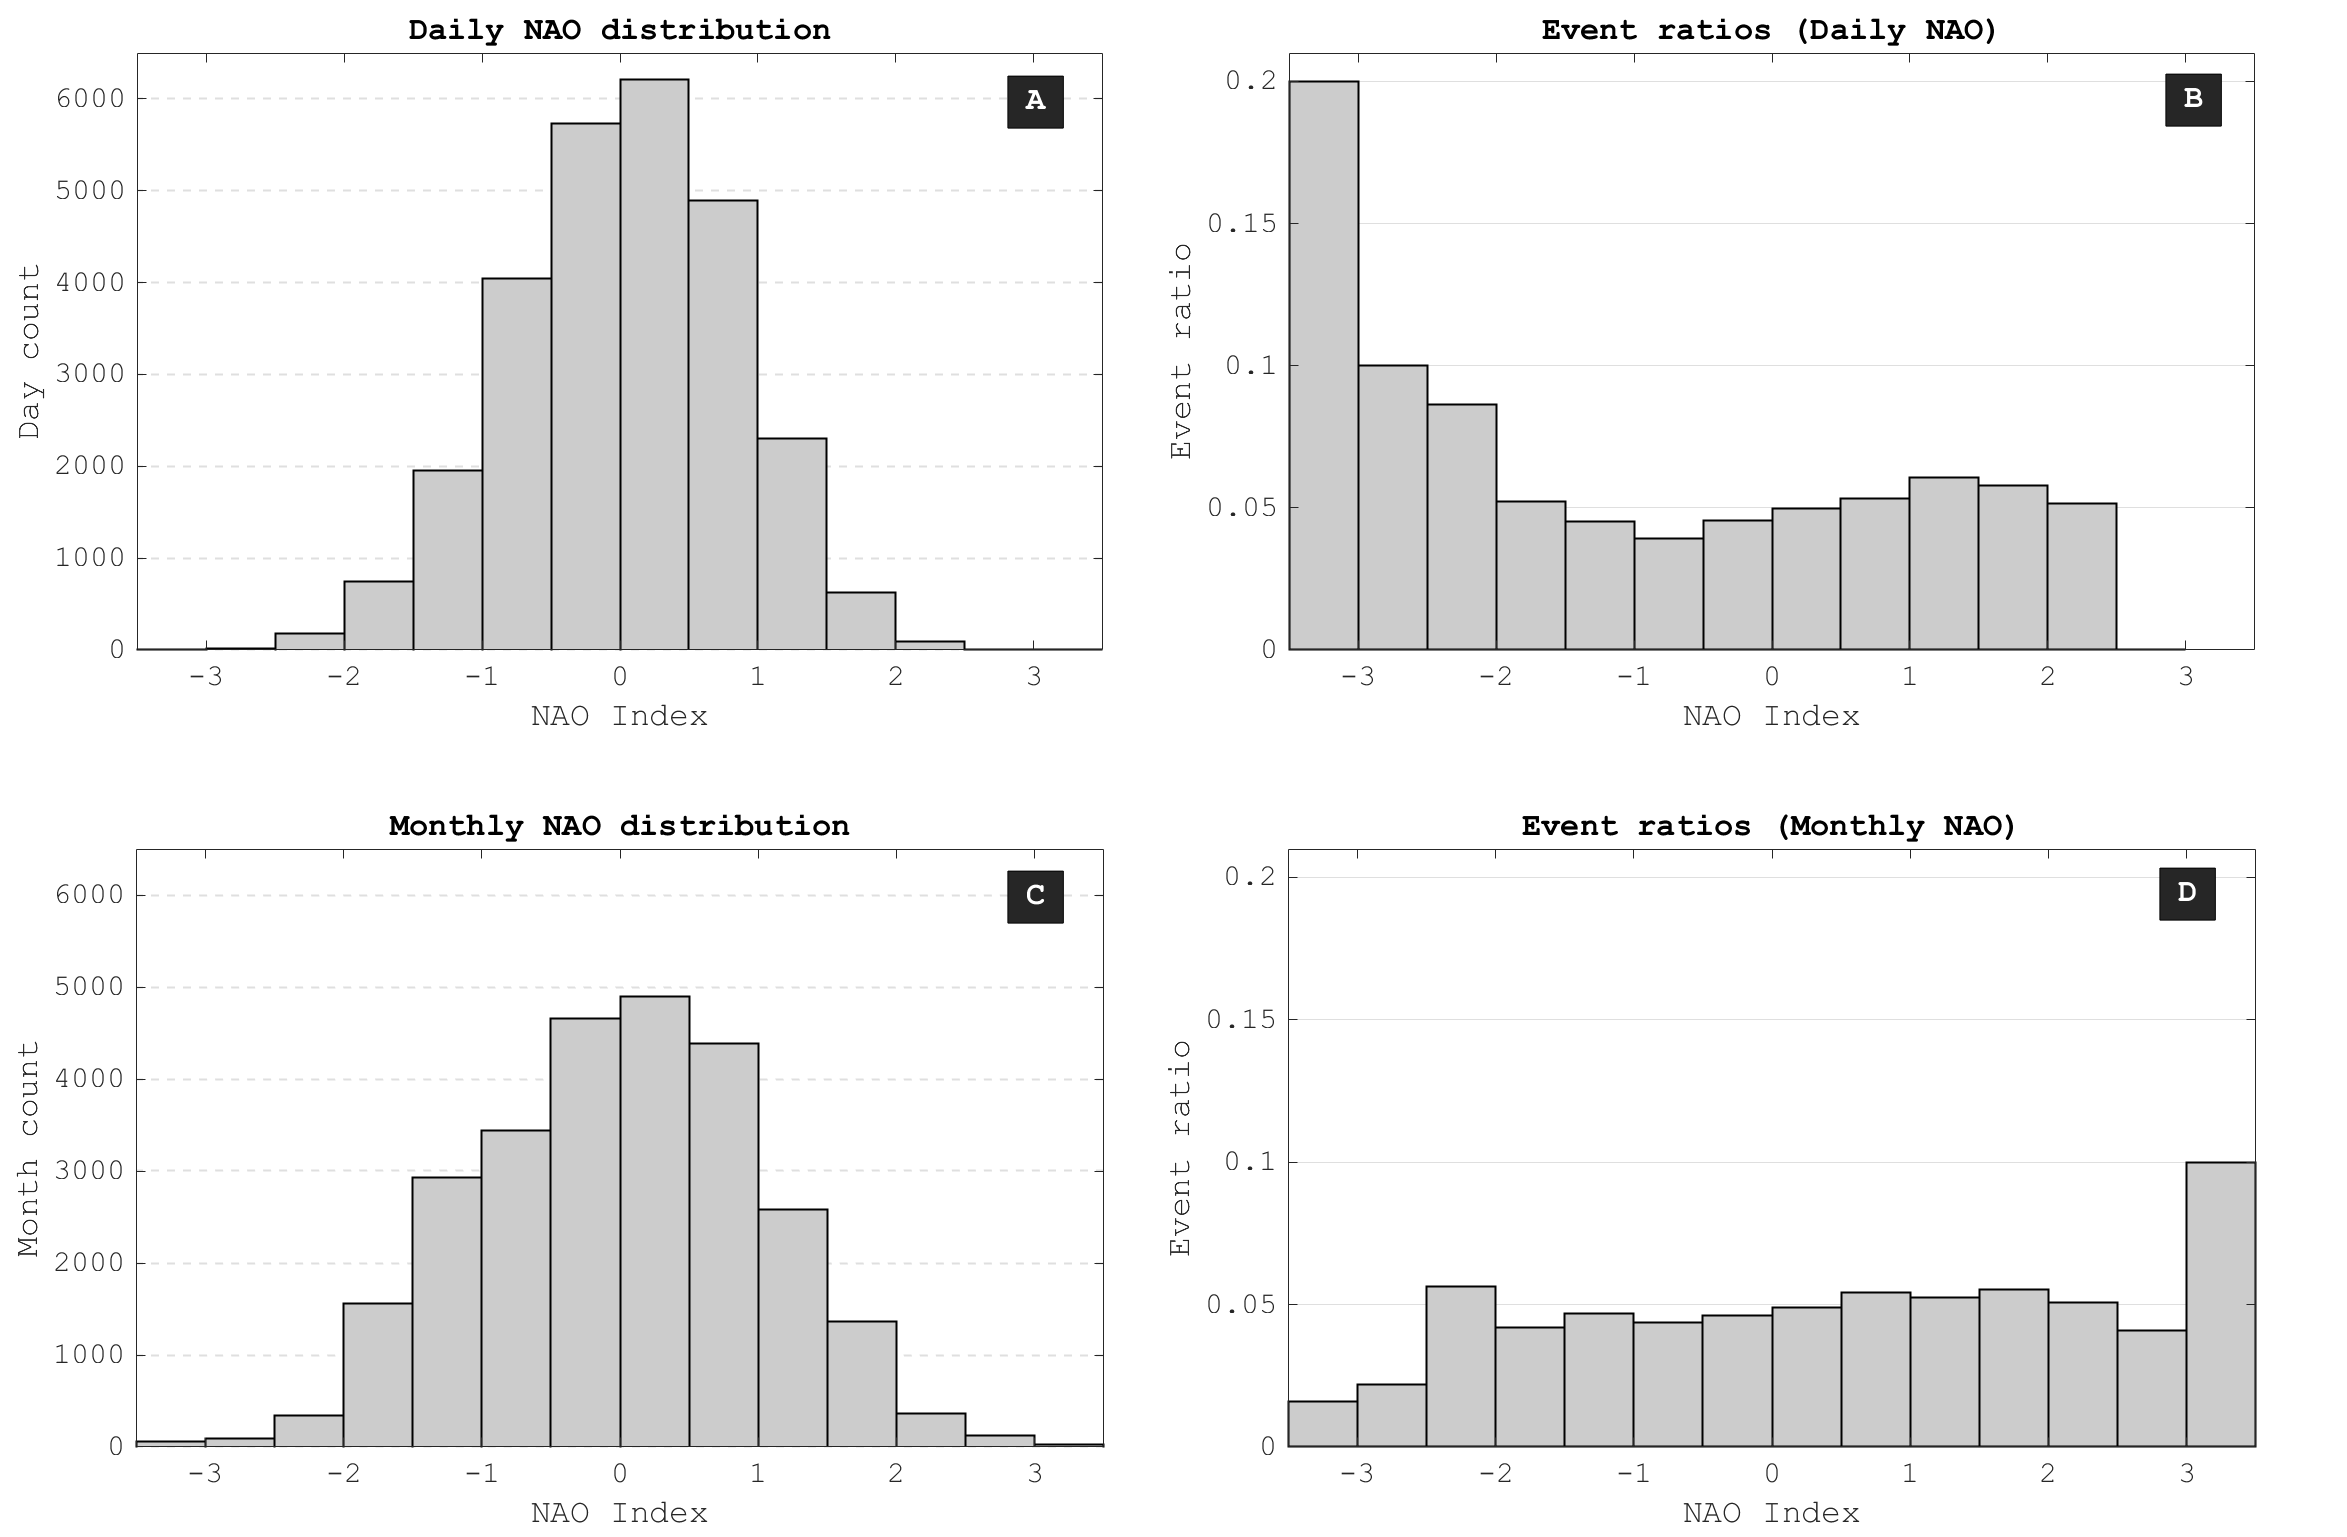
\includegraphics[width=\textwidth]{figures/nao_state_as_four_1.52.png}
            \caption{For this figure, the NAO index of a storm is the index at the day on which the storm begins. The beginning of a storm in this study is defined as 36 hours before the centre (point of highest relative vorticity) of the storm touches land. The NAO index is sourced from the NOAA archive. \textbf{A:} Daily NAO distribution. Represents the number of days that fall within a certain NAO index, starting from -3.5 to 3.5 with steps of 0.5. The peak of the graph lies in the range of 0.0 to 0.5. \textbf{C:} Monthly NAO distribution. The peak of the graph lies in the range 0.0 to 0.5. \textbf{B:} Represents the number of windstorm events associated with a NAO state divided by the total number of days that have had that NAO state. 20\% of days with a NAO index between -3.5 and -3.0 have experienced a windstorm, which is the highest event rate in this figure. The event rates for other NAO instances vary from 5\% to 10\% with no pronounced pattern. \textbf{D:} Monthly Windstorm Event Ratio. 10\% of days with a NAO index between +3.0 and +3.5 have experienced a windstorm, which is the highest event rate in this figure. Event rates for other NAO indices vary between 2\% to 6\% with no pronounced pattern.}
            \label{fig:nao_and_event_rate}
        \end{figure}
        %----------------------------------------------------------------------------------------------------------------------------------

    In Figure \ref{fig:normalized_probability_of_storm_events_with_NAO}, we present the probabalistic distribution of windstorm events by month, further broken down into NAO states. The height of all 12 columns adds up to $1.00$ and they are always stacked so that NAO(-) is on top and NAO (+) at the bottom. The months that have observed the most number of events are December, January, November and February in descending order, while the least events occurred in June, July and August in ascending order. These rates are consistent with previous papers such as those by \cite{Hurrell2003}, \cite{Renggli2011}, and others, where the winter period is associated with a high rate of windstorms, while the summer observes only occasional events. Months with a significant probability of windstorms tend to have events evenly spread between NAO(0) and NAO(-), with a slight tendency towards NAO(0). NAO(-) events are not rare but are consistently less probable than their counterparts.

        % FIGURE 5 ------------------------------------------------------------------------------------------------------------------------
        \sidecaptionvpos{figure}{t}
        \begin{SCfigure}
            \centering
            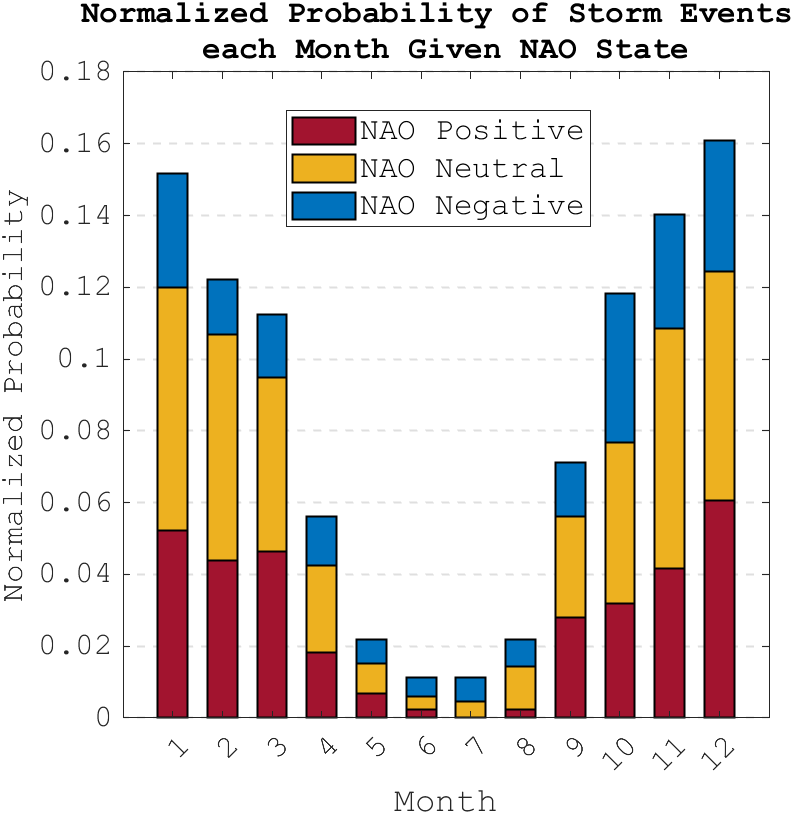
\includegraphics[width=0.6\textwidth]{figures/Normalized Probability of Storm Events Given NAO State(small).png}
            \caption{Represents the probability of observing a windstorm event during each month of the year, sectioned by the NAO index which corresponds to the beggining of the storm. NAO neutral indices are those which belong in the range of -0.5 to 0.5 including. The beginning of a storm in this study is defined as 36 hours before the centre (point of highest relative vorticity) of the storm touches land.}
            \label{fig:normalized_probability_of_storm_events_with_NAO}
        \end{SCfigure}
        %----------------------------------------------------------------------------------------------------------------------------------

    In addition to Figure \ref{fig:normalized_probability_of_storm_events_with_NAO}, we present Figure \ref{fig:averageEnergyPerMonth}. In it we present the average energy of a windstorm event for each month, once again splitting events into categories based on the NAO state they are associated with. Embed on top of each bar is the number of events that go into the respective category in the form 'N =...'. When looking at the boreal winter period of December-January-February, NAO (+) windstorms are significantly more energetic. For the remainder of the year, windstorm energy is more evenly distributed between the three NAO states, with no directly apparent pattern to which is the most energetic.

        % FIGURE 6 ------------------------------------------------------------------------------------------------------------------------
        \begin{figure}
            \centering
            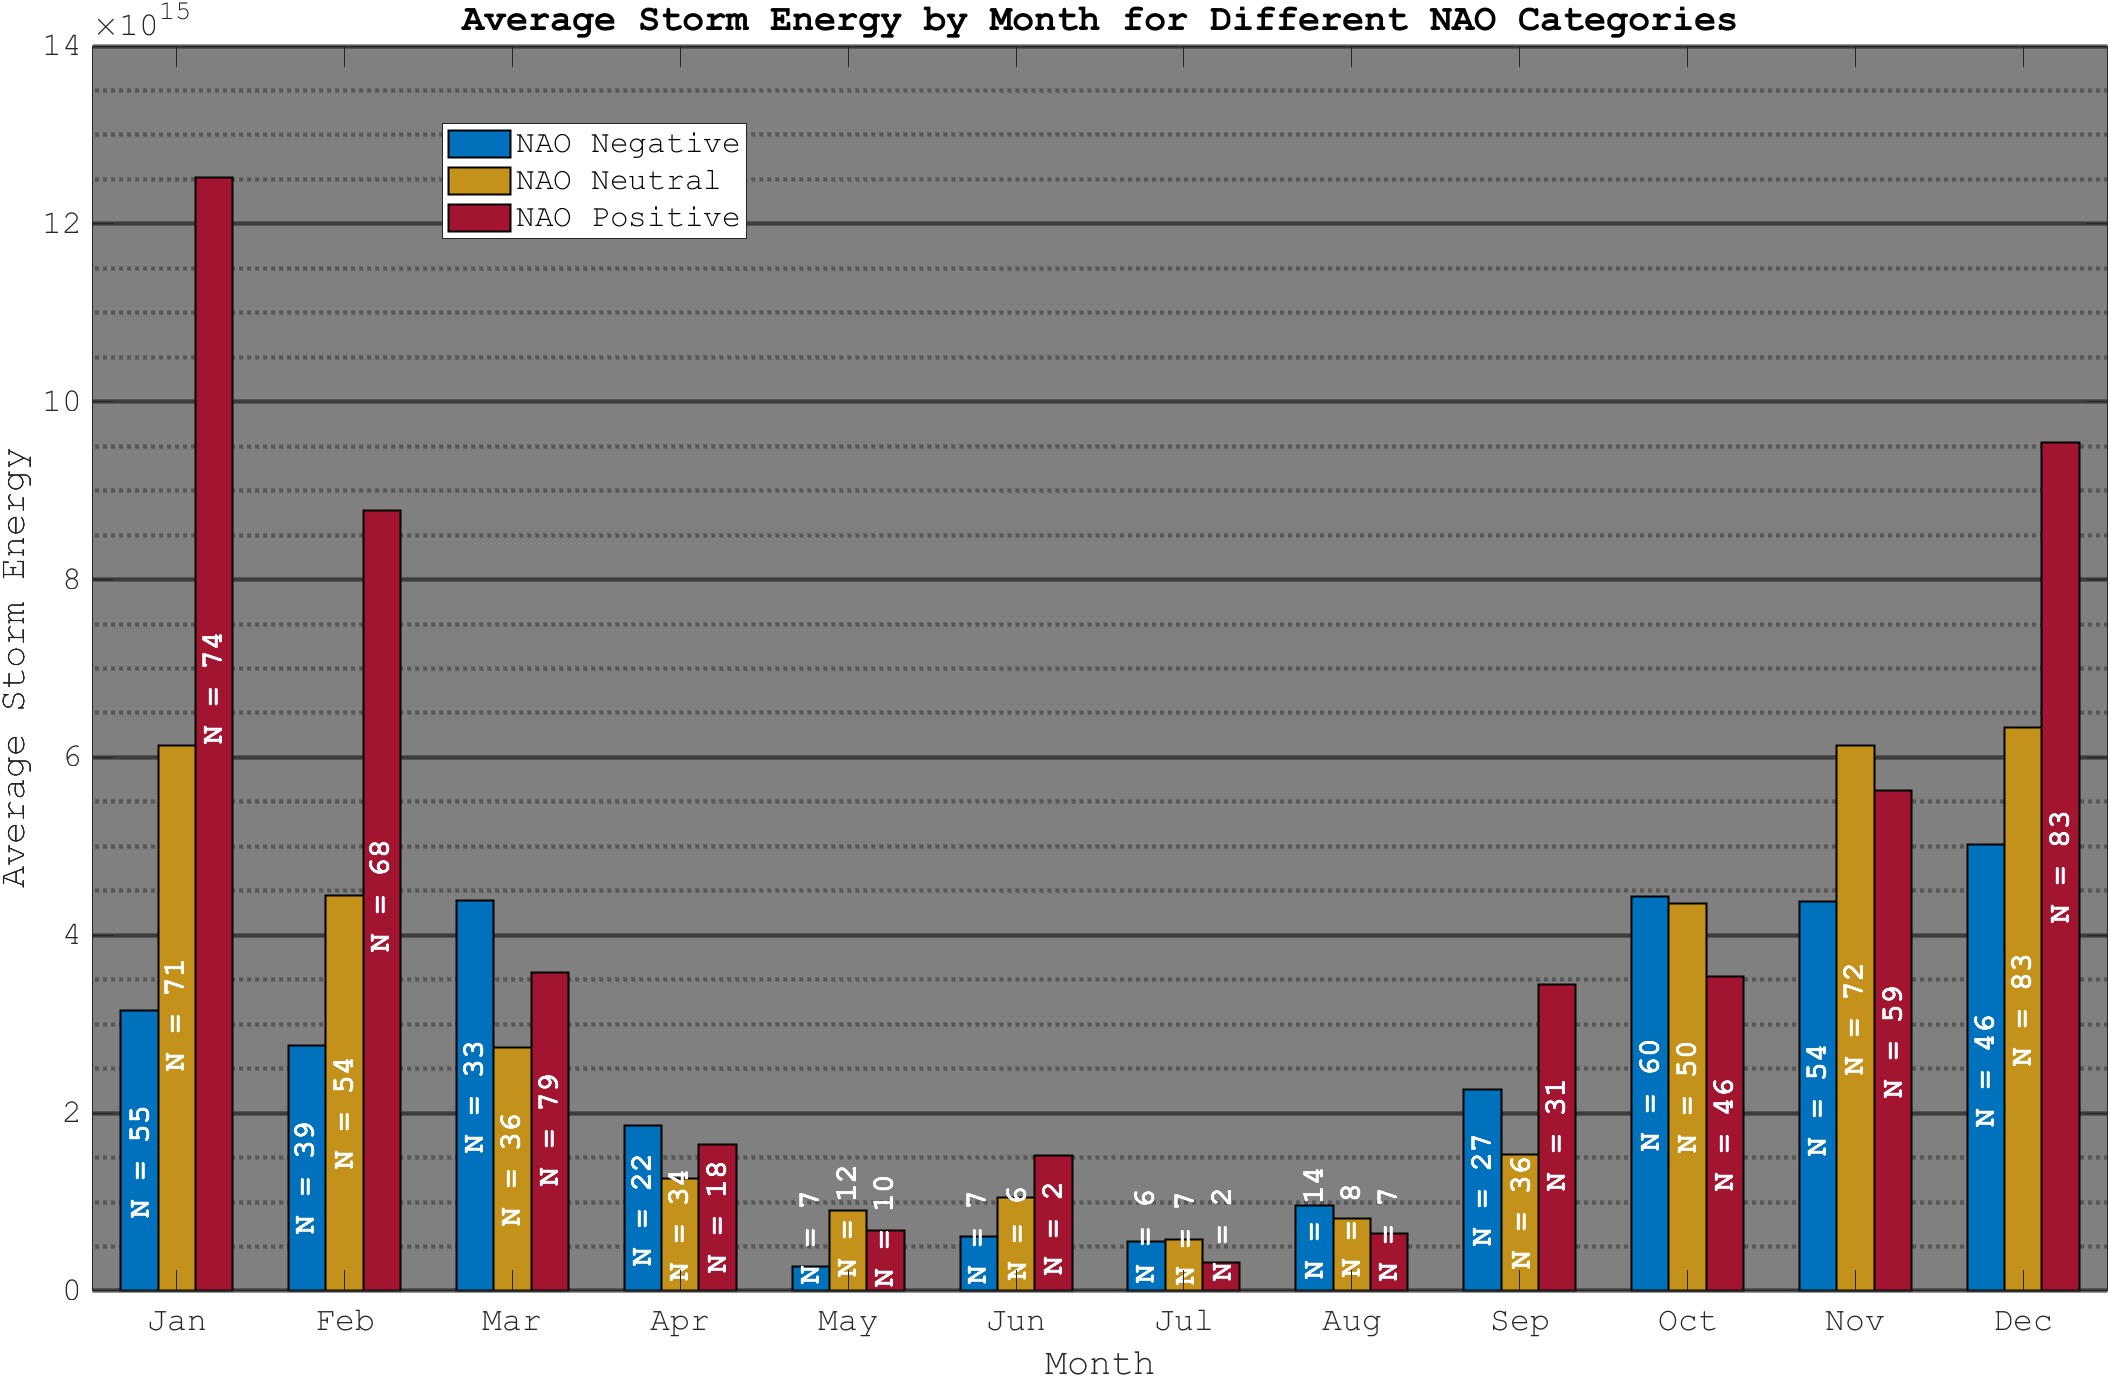
\includegraphics[width=\textwidth]{figures/average_storm_energy_by_month_with_nao_separated.png}
            \caption{Represents the probability of observing a windstorm event during each month of the year, sectioned by the NAO index which corresponds to the beggining of the storm. NAO neutral indices are those which belong in the range of -0.5 to 0.5 including. The beginning of a storm in this study is defined as 36 hours before the centre (point of highest relative vorticity) of the storm touches land.}
            \label{fig:averageEnergyPerMonth}
        \end{figure}
        %----------------------------------------------------------------------------------------------------------------------------------



\FloatBarrier
\section{The Influence of a Longer Dataset on Results}

    Studies on windstorms are limited in terms of data, and depending on the desired accuracy, this range roughly varies from 70 to 30 years. To investigate the effect that different time ranges have on the statistical relationship between windstorms and the NAO, we obtain the exceedance probability of windstorms in western Europe excluding Iceland for three different periods: one where the NAO is predominantly in a positive state, one where it is in a negative state, and one where the average state of the NAO approximates to neutral. Note that the last does not mean that the period is composed of NAO neutral years, but rather NAO negative and NAO positive states are equally represented. 

    The first step is to determine the range for each of the aforementioned periods. To do this, we take the yearly NAO state to be equal to the average of the monthly ones. We present the results in Figure \ref{fig:yearlyNAO}. From it we identify the time between 1950 to 1970 as dominated by a NAO(-) state. 1970 to 2000 is dominated by a NAO(+) state, and we estimate the period from 2000 to 2020 to be balanced.
    
        % FIGURE XTRA #1 ------------------------------------------------------------------------------------------------------------------
        \sidecaptionvpos{figure}{t}
        \begin{SCfigure}
            \centering
            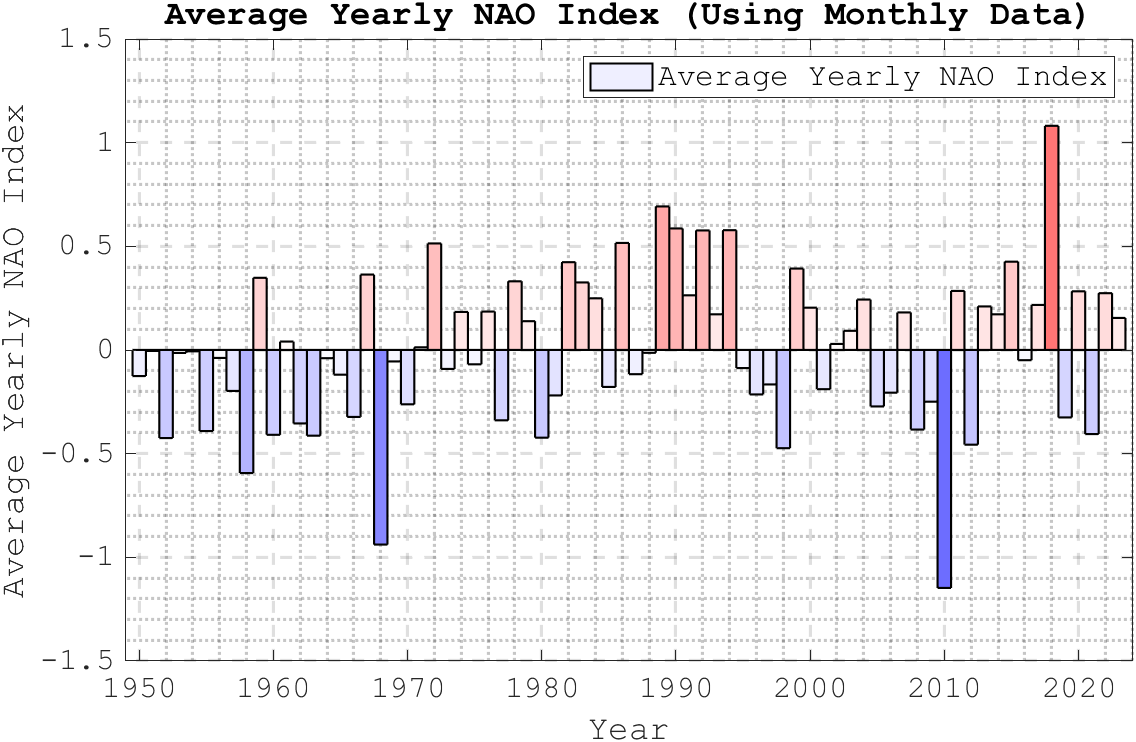
\includegraphics[width=0.7\textwidth]{figures/Average_NAO_Index_Yearly_from_month.png}
            \caption{ Each bar represents the NAO Index for that year as obtained from taking the average of the NAO monthly index.}
            \label{fig:yearlyNAO}
        \end{SCfigure}
        %----------------------------------------------------------------------------------------------------------------------------------

    We also present the EP for the entire period used in this study, beginning in 1950 and ending in 2020 in Figure \ref{fig:EP_Curve_NAO(p,n)_1950-2020}. In it we mark the position of several named storms in the data for added clarity. The figure shows a clear division between NAO(+,0,-) windstorms, with NAO(+) events being the most energetic and NAO(-) events the least energetic. Storms Kyrill and Lothar align with expectations, appearing at the curve's tail. Contrarily, Storm Klaus ranks in the top 40\% of high-energy NAO(-) events, illustrating that a storm's perceived impact isn't solely determined by its strength, but also by its trajectory, such as whether it passes over open land or populated areas.

        % FIGURE 4 ------------------------------------------------------------------------------------------------------------------------
        \sidecaptionvpos{figure}{t}
        \begin{SCfigure}
            \centering
            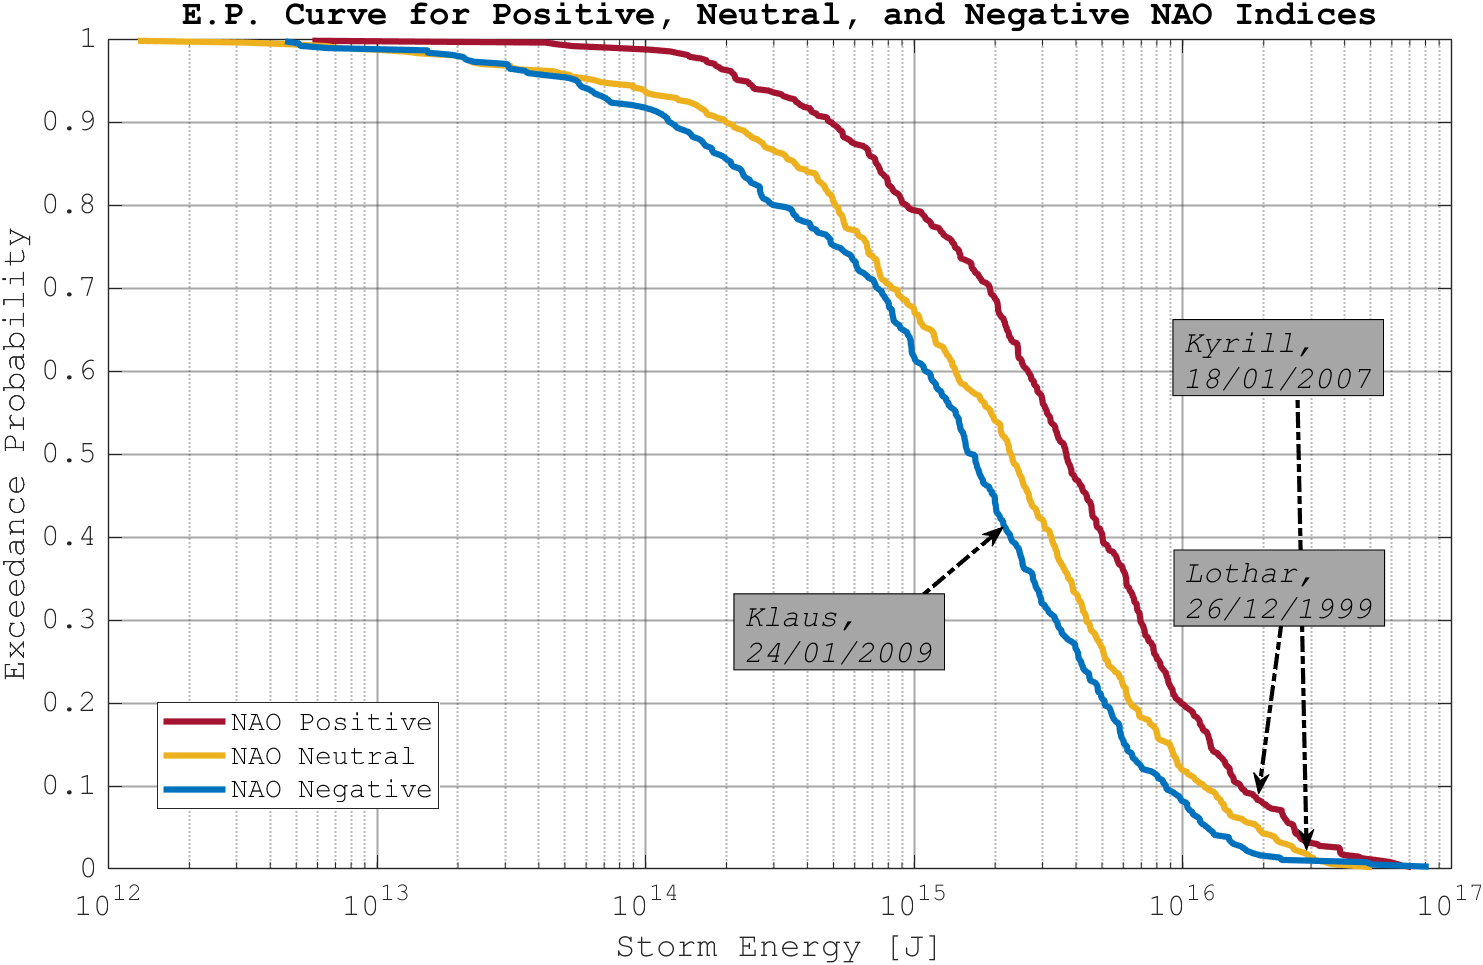
\includegraphics[width=0.7\textwidth]{figures/EP Curve NAO(p,n), 1950-2020(small)_with_neutral_nao.png}
            \caption{Exceedance probability curve for positive, negative and neutral NAO. Data are obtained from windstorm energy estimations as presented in this study and the NOAA NAO index database for the period of 1950 to 2020. The position of some named storms is shown for perspective.}
            \label{fig:EP_Curve_NAO(p,n)_1950-2020}
        \end{SCfigure}
        %----------------------------------------------------------------------------------------------------------------------------------

        % TABLE 1 -------------------------------------------------------------------------------------------------------------------------
        \begin{table}
        \centering
        \resizebox{\textwidth}{!}{%
        \begin{tabular}{ccccccccccc}
         &
          \multicolumn{1}{c|}{} &
          \multicolumn{3}{c|}{\textbf{N}} &
          \multicolumn{3}{c|}{\textbf{Mean Energy {[}$10^{15}$J{]}}} &
          \multicolumn{3}{c}{\textbf{Median Energy {[}$10^{15}$J{]}}} \\
         &
          \multicolumn{1}{c|}{D.S.} &
          \cellcolor[HTML]{FFCCC9}\textbf{NAO(+)} &
          \cellcolor[HTML]{FFFFC7}\textbf{NAO(0)} &
          \multicolumn{1}{c|}{\cellcolor[HTML]{ECF4FF}\textbf{NAO(-)}} &
          \cellcolor[HTML]{FFCCC9}\textbf{NAO(+)} &
          \cellcolor[HTML]{FFFFC7}\textbf{NAO(0)} &
          \multicolumn{1}{c|}{\cellcolor[HTML]{ECF4FF}\textbf{NAO(-)}} &
          \cellcolor[HTML]{FFCCC9}\textbf{NAO(+)} &
          \cellcolor[HTML]{FFFFC7}\textbf{NAO(0)} &
          \cellcolor[HTML]{ECF4FF}\textbf{NAO(-)} \\
        {\color[HTML]{00009B} 1950:1970} &
          \multicolumn{1}{c|}{{\color[HTML]{00009B} -'ve}} &
          \cellcolor[HTML]{FFCCC9}{\color[HTML]{00009B} 98} &
          \cellcolor[HTML]{FFFFC7}{\color[HTML]{00009B} 126} &
          \multicolumn{1}{c|}{\cellcolor[HTML]{ECF4FF}{\color[HTML]{00009B} 150}} &
          \cellcolor[HTML]{FFCCC9}{\color[HTML]{00009B} 5.2} &
          \cellcolor[HTML]{FFFFC7}{\color[HTML]{00009B} 5.2} &
          \multicolumn{1}{c|}{\cellcolor[HTML]{ECF4FF}{\color[HTML]{00009B} 3.7}} &
          \cellcolor[HTML]{FFCCC9}{\color[HTML]{00009B} 2.8} &
          \cellcolor[HTML]{FFFFC7}{\color[HTML]{00009B} 2.8} &
          \cellcolor[HTML]{ECF4FF}{\color[HTML]{00009B} 1.5} \\
        {\color[HTML]{680100} 1970:2000} &
          \multicolumn{1}{c|}{{\color[HTML]{680100} +'ve}} &
          \cellcolor[HTML]{FFCCC9}{\color[HTML]{680100} 224} &
          \cellcolor[HTML]{FFFFC7}{\color[HTML]{680100} 207} &
          \multicolumn{1}{c|}{\cellcolor[HTML]{ECF4FF}{\color[HTML]{680100} 152}} &
          \cellcolor[HTML]{FFCCC9}{\color[HTML]{680100} 7.5} &
          \cellcolor[HTML]{FFFFC7}{\color[HTML]{680100} 4.4} &
          \multicolumn{1}{c|}{\cellcolor[HTML]{ECF4FF}{\color[HTML]{680100} 3.8}} &
          \cellcolor[HTML]{FFCCC9}{\color[HTML]{680100} 3.8} &
          \cellcolor[HTML]{FFFFC7}{\color[HTML]{680100} 2.2} &
          \cellcolor[HTML]{ECF4FF}{\color[HTML]{680100} 2.0} \\
        {\color[HTML]{656565} 2000:2020} &
          \multicolumn{1}{c|}{{\color[HTML]{656565} -/-}} &
          \cellcolor[HTML]{FFCCC9}{\color[HTML]{656565} 153} &
          \cellcolor[HTML]{FFFFC7}{\color[HTML]{656565} 133} &
          \multicolumn{1}{c|}{\cellcolor[HTML]{ECF4FF}{\color[HTML]{656565} 82}} &
          \cellcolor[HTML]{FFCCC9}{\color[HTML]{656565} 7.1} &
          \cellcolor[HTML]{FFFFC7}{\color[HTML]{656565} 4.3} &
          \multicolumn{1}{c|}{\cellcolor[HTML]{ECF4FF}{\color[HTML]{656565} 2.5}} &
          \cellcolor[HTML]{FFCCC9}{\color[HTML]{656565} 3.8} &
          \cellcolor[HTML]{FFFFC7}{\color[HTML]{656565} 2.2} &
          \cellcolor[HTML]{ECF4FF}{\color[HTML]{656565} 1.0} \\ \hline
        1950:2020 &
           &
          \cellcolor[HTML]{FFCCC9}465 &
          \cellcolor[HTML]{FFFFC7}462 &
          \cellcolor[HTML]{ECF4FF}364 &
          \cellcolor[HTML]{FFCCC9}6.9 &
          \cellcolor[HTML]{FFFFC7}4.6 &
          \cellcolor[HTML]{ECF4FF}3.5 &
          \cellcolor[HTML]{FFCCC9}3.7 &
          \cellcolor[HTML]{FFFFC7}2.3 &
          \cellcolor[HTML]{ECF4FF}1.6
        \end{tabular}%
        }
        \caption{Table with statistical information about Figures \ref{fig:EP19501970}, \ref{fig:EP19702000}, \ref{fig:EP20002020} and \ref{fig:EP_Curve_NAO(p,n)_1950-2020}. Dominant state for period given in D.S. column}
        \label{tab:eptable}
        \end{table}
        %----------------------------------------------------------------------------------------------------------------------------------

    In Figures \ref{fig:EP19501970}, \ref{fig:EP19702000} and \ref{fig:EP20002020} we present the EP curves for the earlier defined periods. Statistics such as the number of members, mean and median energy can be found in Table \ref{tab:eptable}. 

        % FIGURE 12 -----------------------------------------------------------------------------------------------------------------------
        \begin{figure}[ht]
            \begin{minipage}[t]{0.7\textwidth}
                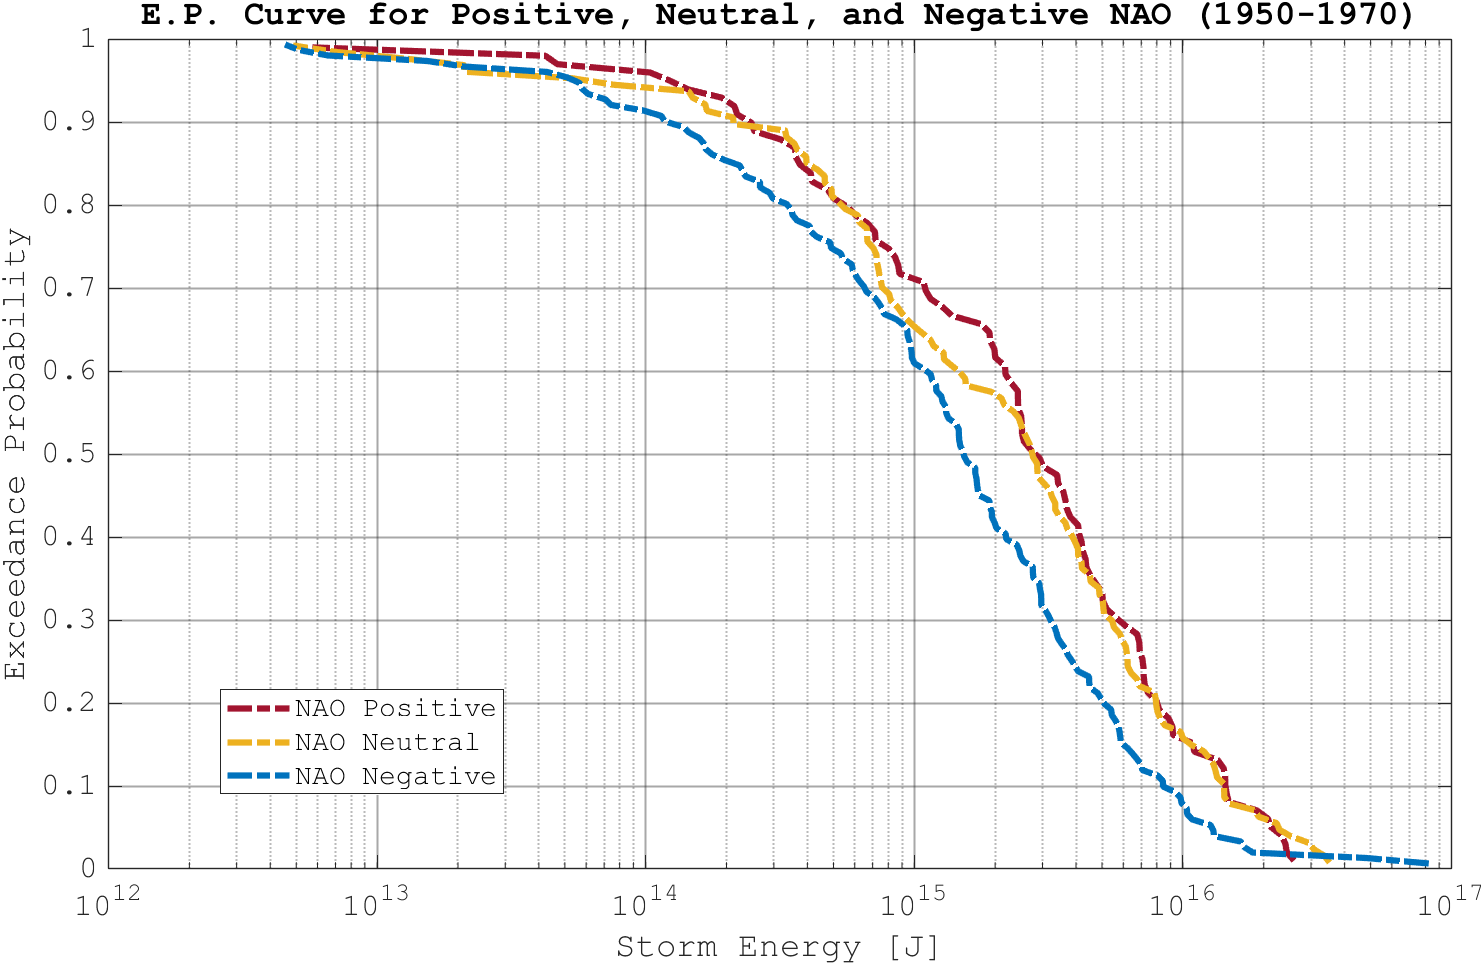
\includegraphics[width=\textwidth]{figures/EP_curve_1950_1970.png}
                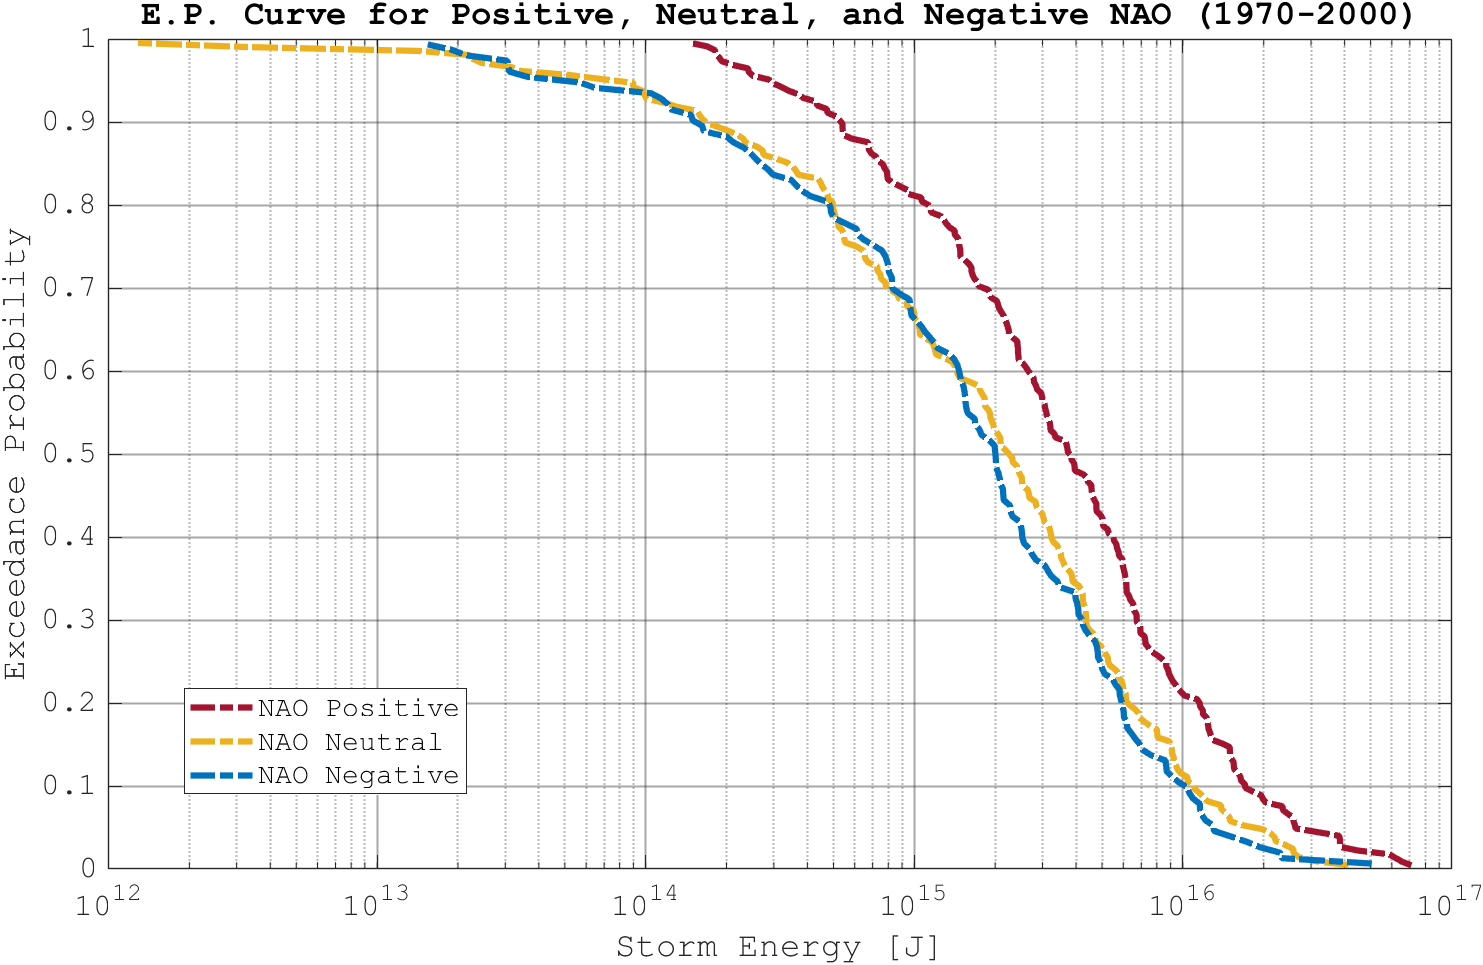
\includegraphics[width=\textwidth]{figures/EP_curve_1970_2000.png}
                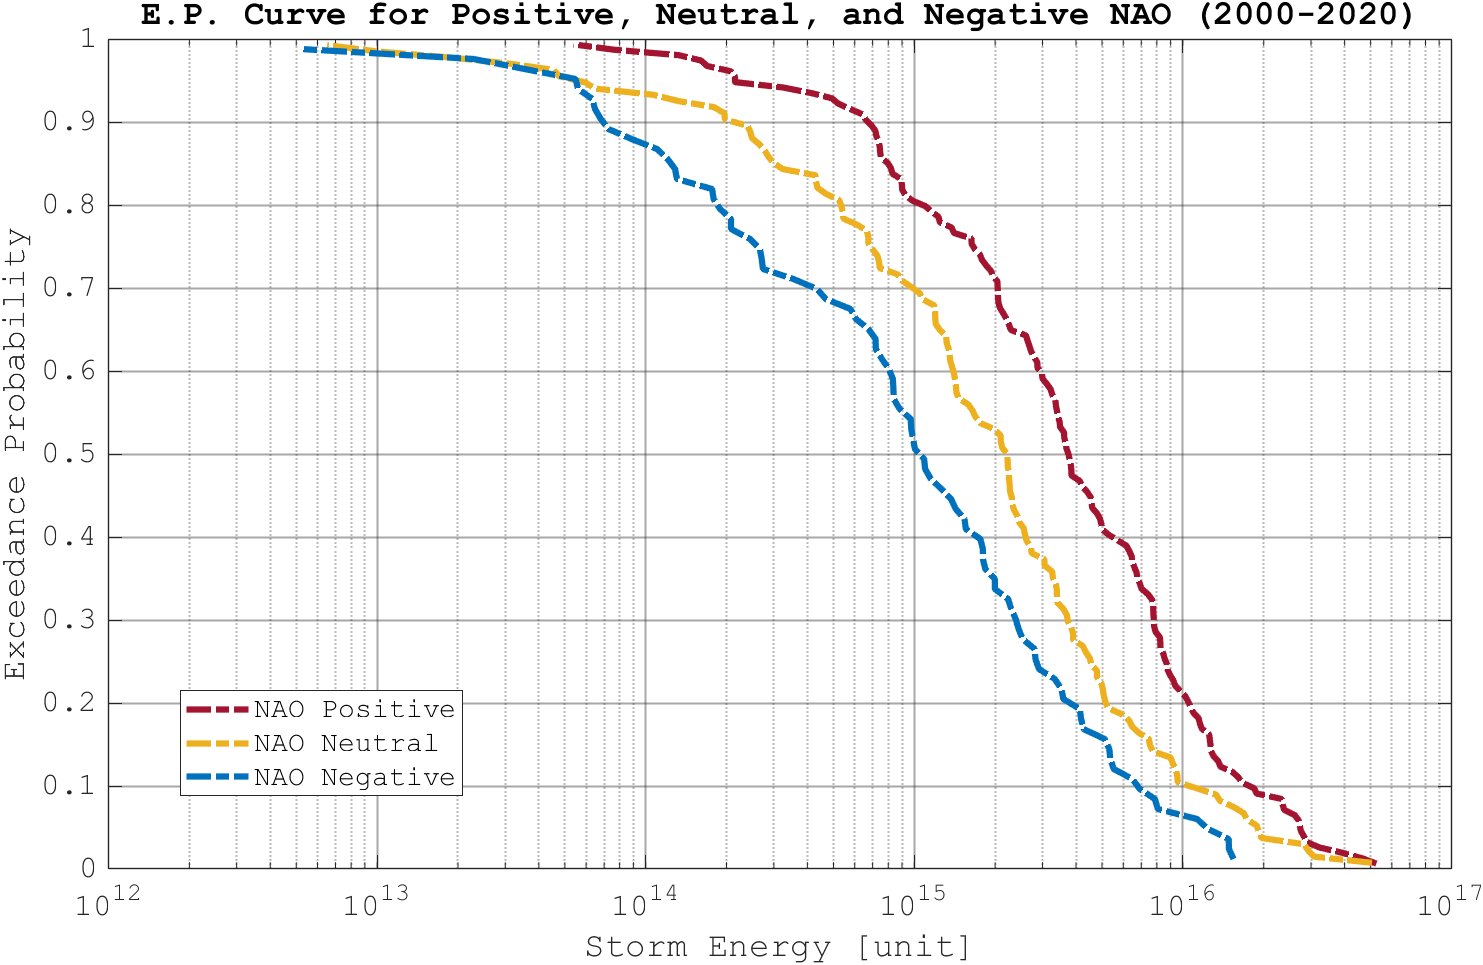
\includegraphics[width=\textwidth]{figures/EP_curve_2000_2020.png}
            \end{minipage}
            \hfill  % Fill horizontal space
            \begin{minipage}[t]{0.29\textwidth}
                \vspace*{-215pt}  % Move the start of the caption upwards. You might need to adjust this value.
                \caption{Exceedance probability curve for positive, negative and neutral NAO for the period 1950 to 1970. Mean Energy in PetaJoules: NAO(+)~5.2, NAO(0)~5.2, NAO(-)~3.7}
                \label{fig:EP19501970}
                \vspace*{110pt}  % Increase space between captions. You might need to adjust this value.
                \caption{Exceedance probability curve for positive, negative and neutral NAO for the period 1970 to 2000. Mean Energy in PetaJoules: NAO(+)~7.5, NAO(0)~4.4, NAO(-)~3.8}
                \label{fig:EP19702000}
                \vspace*{110pt}  % Increase space between captions. You might need to adjust this value.
                \caption{Exceedance probability curve for positive, negative and neutral NAO for the period 2000 to 2020. Mean Energy in PetaJoules: NAO(+)~7.1, NAO(0)~4.3, NAO(-)~2.5}
                \label{fig:EP20002020}
            \end{minipage}
        \end{figure}
        %----------------------------------------------------------------------------------------------------------------------------------

\FloatBarrier
\section{The Influence of the NAO State on Windstorm Paths in Europe}

    To investigate the path taken by storms during different states of the NAO we produce two sets of figures. In one we present the distribution of energy from our windstorm dataset divided into the country over which the energy was released. The set contains this for two time periods - boreal winter and boreal summer given in Figures \ref{fig:DJF_Tot_Eng_by_cunt} and \ref{fig:JJA_Tot_Eng_by_cunt}, respectively. Note that the energy during boreal summer is two orders of magnitude lower than that during boreal winter. During the December to January period windstorm energy is concentrated in the UK, Spain, Belgium, and Norway, in that order. During the June to August period, windstorm energy is highest in the UK, Denmark, Norway, and Belgium.
    
        % FIGURE 7 + 8 --------------------------------------------------------------------------------------------------------------------
        \begin{figure}[ht]
            \begin{minipage}[t]{0.59\textwidth}
                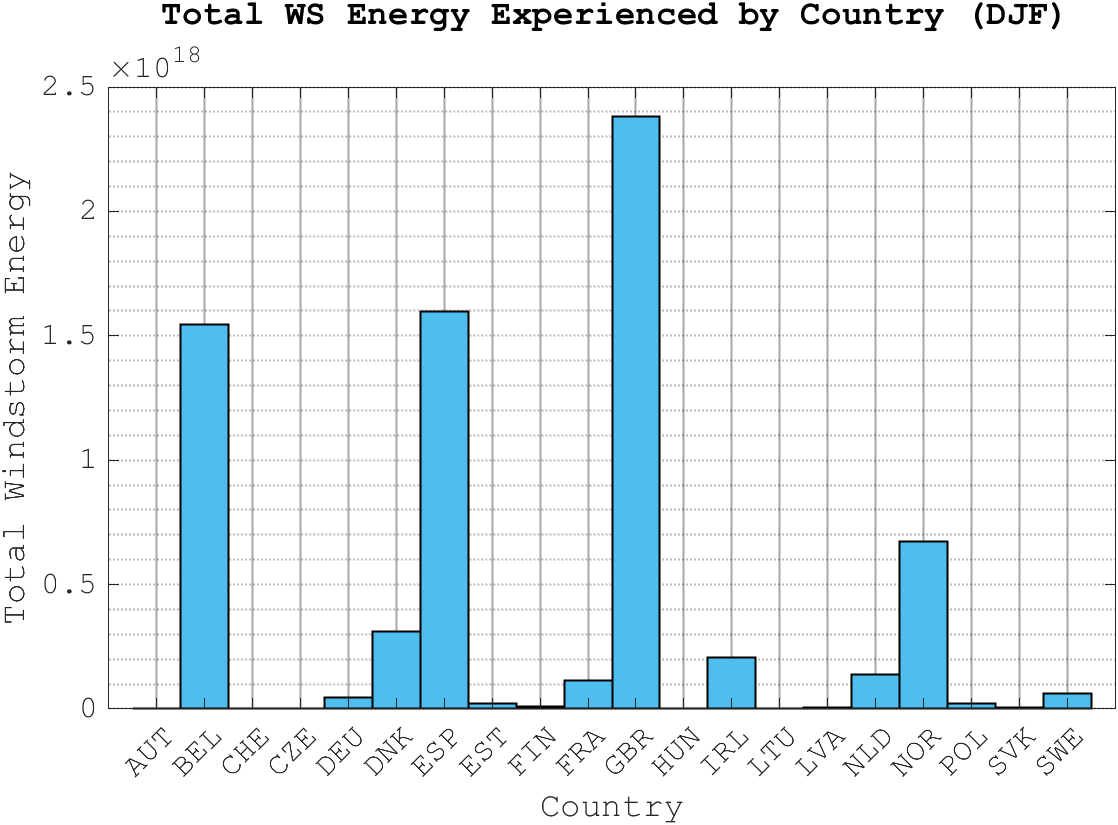
\includegraphics[width=\textwidth]{figures/Total Energy of WS DJF.png}
                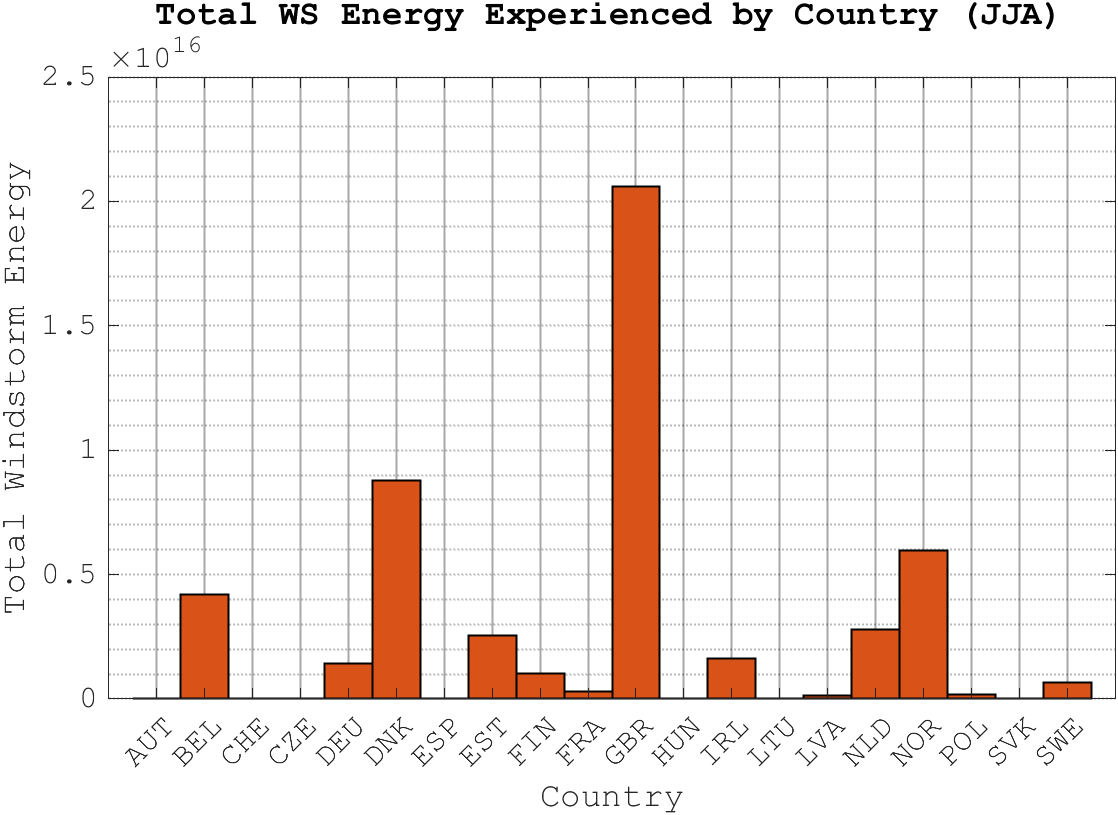
\includegraphics[width=\textwidth]{figures/Total Energy of WS JJA.png}
            \end{minipage}
            \hfill  % Fill horizontal space
            \begin{minipage}[t]{0.4\textwidth}
                \vspace*{-190pt}  % Move the start of the caption upwards. You might need to adjust this value.
                \caption{Represents the sum of WS energy recorded within the area of each country during Boreal Winter - December, January and February.}
                \label{fig:DJF_Tot_Eng_by_cunt}
                \vspace*{140pt}  % Increase space between captions. You might need to adjust this value.
                \caption{Represents the sum of WS energy recorded within the area of each country during Boreal Summer - June, July, August.}
                \label{fig:JJA_Tot_Eng_by_cunt}
            \end{minipage}
        \end{figure}
        %----------------------------------------------------------------------------------------------------------------------------------

    The second set of figures is presented in Figures \ref{fig:epcurvescountry}A-H. In them the exceedance probabilities of European countries along the east coast are presented. It begins from Spain in Figure \ref{fig:epcurvescountry}A, which is the southernmost country in the dataset of this study, and continues north. Along with the figure for each country, information is shown on the number of events that make up a curve. This is important when comparing the EP in a country versus the information in Figures \ref{fig:DJF_Tot_Eng_by_cunt} and \ref{fig:JJA_Tot_Eng_by_cunt} and Figures \ref{fig:naopostitivemap}, \ref{fig:naoneutralmapo} and \ref{fig:naonegativemapenter-label}. 

        % FIGURE 9 + 10 + 11 --------------------------------------------------------------------------------------------------------------
        \begin{figure}
            \centering
            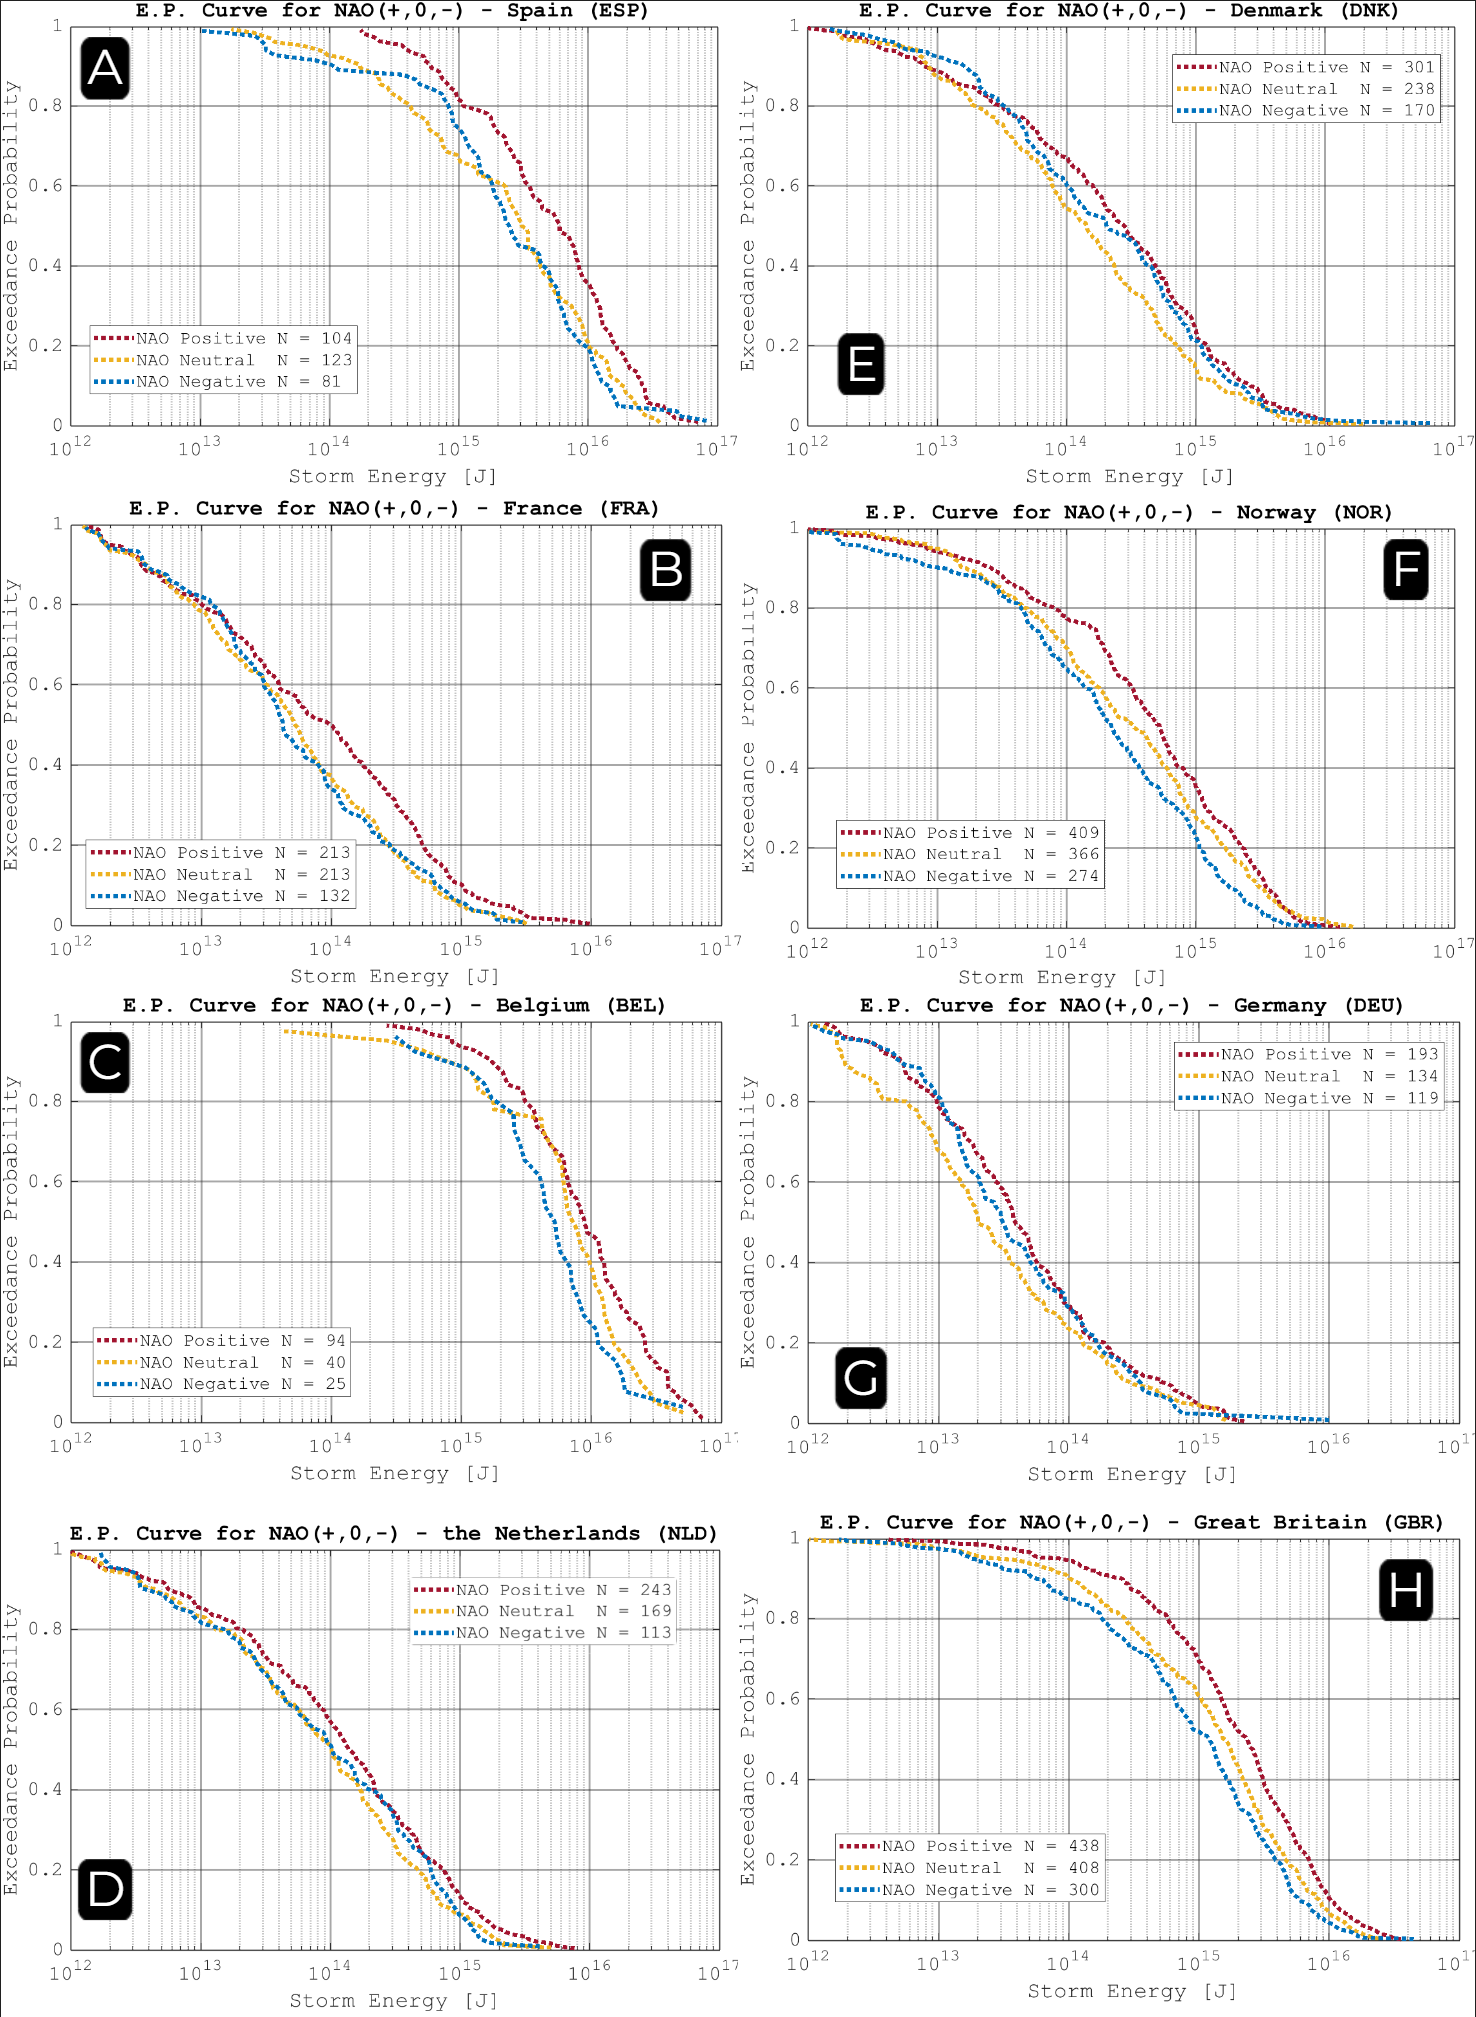
\includegraphics[width=\textwidth]{figures/epcurvescountry.png}
            \caption{Exceedance Probability for countries at the Western European border.}
            \label{fig:epcurvescountry}
        \end{figure}
        %----------------------------------------------------------------------------------------------------------------------------------
    







    
    
    




% CHAPTER 6
\chapter{Discussion of Results, Conclusions and Future work}
    \section{Discussion}

    \subsection{Risk of European Windstorm during NAO Neutral Index}

        In Figures \ref{fig:storm_count_vs_daily_nao} and \ref{fig:storm_count_vs_monthly_nao} we presented the number of windstorms associated with different states of the NAO. Our results support the findings of \cite{https://doi.org/10.1002/joc.1982} and \cite{https://doi.org/10.1002/2014GL059647}. In both cases, using daily or monthly NAO values, the maximum number of storms was observed in the range where the NAO index was between 0.0 and 0.5, although when using monthly indices the distribution is less pronounced than its daily index counterpart. This is due to the natural smoothing that occurs when using a value that encapsulates a longer timeframe. Daily values are more nuanced but can be noisy, whereas monthly values are smoother but also more reliable. As described in Chapter 3, the way we determine the NAO state associated with a windstorm is by taking the one at the start of an event, defined as 36 hours before the point of highest vorticity moves over land anywhere in western Europe, including the UK and excluding Iceland. Because 36 hours is an arbitrary period that was found to best work with the algorithm to define windstorm events, there is a degree of uncertainty as to how accurately the state of the NAO is defined. By repeating statistical analysis using monthly values, we minimise this uncertainty as the likelyhood that an event had its starting time out by 15 days (the average length of time an event would be from a different month) is insignifficant.

        Next, we determine the distribution of the NAO states themselves, given in Figures \ref{fig:nao_and_event_rate}A and \ref{fig:nao_and_event_rate}C, to investigate the relationship between daily / monthly NAO and the frequency of windstorms. The figures show a spread of NAO states nearly identical in shape to the spread of events in Figures \ref{fig:storm_count_vs_daily_nao} and \ref{fig:storm_count_vs_monthly_nao}. The distribution is not dissimilar to that produced by an oscillator between -3.5 and 3.5 with a small positive bias. If we obtain the ratio of windstorm events associated with a particular NAO state to the number of days with that NAO state, we obtain an even spread, as presented in Figures \ref{fig:nao_and_event_rate}B and \ref{fig:nao_and_event_rate}D. The daily rates vary between 5 and 10\%, while the monthly rates are smoother and vary between 4 and 6\%. At the tail of the distribution, for events associated with an NAO index of magnitude larger than 3, we observe a high probability that days with that NAO state will observe a windstorm - 20\% in Figure \ref{fig:nao_and_event_rate}B, however, the uncertainty is high in that range, as the number of events ($<5$), and the number of days of that state ($<30$) is very low compared to the duration of the study (70 years). We conclude that the state of the NAO, when estimated on the daily or monthly, has not displayed a significant relation to the frequency of windstorms in western Europe.

        A different angle and a similar conclusion is obtained when we consider the overlaying state of the NAO. In Section 5.2 we discuss the influence of the period and length of a dataset on the statistical relationship between windstorms and the NAO. Therein are Figure \ref{fig:yearlyNAO} and Table \ref{tab:eptable}. In the figure we present the yearly NAO, from 1950 to 2020, as the average of the monthly NAO. We are able to identify long periods of time when the NAO has a tendency towards the positive or negative, such as the range from 1950 to 1970 when the NAO was biased towards the negative and the range from 1970 to 2000 when the NAO was biased towards a positive state. The predisposition is not large in magnitude and is often $<5$, which we would normally classify as NAO neutral in the case of daily and monthly values; however, since these are the average of many values over a long period of time, we expect a more subtle variance and as such we focus on the sign and place less importance over the magnitude. 
        In Table \ref{tab:eptable} we present information relevant to the exceedance probability curves generated for the different periods we can identify in Figure \ref{fig:yearlyNAO}. We also list the number of events, split by their associated NAO state, that go into each period. In the previous paragraphs we discussed how the monthly NAO state has no relation to the frequency of windstorms, however, in Table \ref{tab:eptable} we record a significantly larger number of NAO(+) windstorms per year (7.5) during the positively biased period of 1970 to 2000 in comparison to the number of NAO(+) windstorms per year (4.9) during the negatively biased period of 1950 to 1970. 1970 to 2000 also observes a slightly higher number of NAO(0) events per year (6.9), compared to 1950 to 1970 (6.3). The opposite is true for NAO(-) events with the period of 1970-2000 observing only 5.1 windstorms/year of that type versus 7.5 windstorms/year during 1950-1970. Further research is needed to determine exactly what effect an unbiased period would have on windstorm frequency, as the above findings cannot distinguish a long enough period where the yearly average is close to 0. Note that the period from 2000 to 2020 is not truly neutral; it merely contains an even mixture of positive and negative years.

        The spread of events for the two periods discussed also differs from the spread of events in Figure \ref{fig:storm_count_vs_daily_nao} (we use daily NAO values to produce EP curves and therefore the table). Illustrated in the figure, NAO(+) events make up 34\% of events, NAO(0) - 44\%, and NAO(-) make up 22\%: NAO(+/0/-)=34/44/22. In the negatively biased period of 1950-1970 this ratio is NAO(+/0/-)=26/34/40 and in the positively biased 1970-2000 the ratio is NAO(+/0/-)=38/35/26. This shows that the distribution of event frequency has its maximum in the same NAO state as the bias of the period in which it resides. This is exactly what we would expect to see in a world where windstorm events were not related to the state of the NAO. An oscillator with its maxima in a particular state would most likely exist in that state during the occurrence of a separate event, with increasingly diminishing probability towards the minima. In this study, the oscillator is the NAO with its maxima determined by the period over which it is observed and constrained by the minima -3.5 and 3.5.

        In Figure \ref{fig:normalized_probability_of_storm_events_with_NAO} we observe a much more significant connection relating the frequency and seasonality of the windstorms. Windstorms in western Europe are most likely during the winter months of November to February and least likely in the summer months from May to August. This agrees with the consensus of previous studies in which the December-January period is established as the storm season \cite{Hurrell2003}, \cite{Pinto2009}, \cite{Palin2016}, \cite{Degenhardt2023}. 
        The distribution of events by NAO state for each month is similar to the distribution given in Figure \ref{fig:storm_count_vs_daily_nao}, which agrees with our conclusions so far. 

        So far we have concluded that through our analysis we have produced no statistical connection between the state of the NAO and the frequency of windstorm events. Strong corellation is observed between windstorm frequency and seasonality. Next, we will investigate the intensity of windstorms and their relation to the NAO state. In Figure \ref{fig:averageEnergyPerMonth} we present the average energy of windstorms for each month, split into their corresponding NAO states. A strong relation of windstorm severity is observed with both seasonality and the state of the NAO. The most energetic windstorms occur during the winter months. During those months, the most violent of storms occurred during a positive NAO, followed by neutral NAO events and with negative NAO events being the least energetic. During the summer months, this relationship between windstorm energy and the state of the NAO is not prominent, however, the number of events in each category is largely $<10$. In addition, if we consider the low energies of storms during that period, it becomes difficult to arrive at a meaningful conclusion.
        High-energy winter windstorm events during a positive NAO are also highlighted in Figure \ref{fig:EP_Curve_NAO(p,n)_1950-2020}, which shows the exceedance probability of windstorms from 1950 to 2020. As mentioned above, NAO(+) windstorms are most energetic, followed by NAO(0) and NAO(-). We conclude that NAO is an important driver of windstorm strength during the winter season. Seasonal effects also play an important role in the frequency and severity of windstorms.
    
    \subsection{The Influence of a Longer Dataset on Results}

        In the preceding section, we presented the annual NAO patterns as shown in Figure \ref{fig:yearlyNAO}. We identified three distinct periods: 1950-1970, characterised by a negative NAO bias; 1970-2000, marked by a positive NAO bias; and 2000-2020, featuring a balanced mix of both negative and positive states. We also introduced the exceedance probability (EP) curve, Figure \ref{fig:EP_Curve_NAO(p,n)_1950-2020}, covering the entire length of the study - 1950-2020. When discussing the probability that a windstorm event will take place during various states of the NAO, we also showed that the distribution of events associated with a particular NAO index is the result of the statistical distribution of the NAO states during the relevant period. And the statistical distribution is directly tied to the time frame over which it is taken, e.g. from 1970 to 2000 the NAO was predominantly positive, leading to the result in Table \ref{tab:eptable}, where the majority of windstorms during that time frame occurred while the NAO was in a positive state. This illustrates the importance of considering the period during which a study makes its statistical analysis. 

        We also established that NAO(+) events tend to be significantly more energetic than their counterparts, particularly during the winter season, which is when the majority of windstorms occur. Thus, we would expect a period with a predominantly positive NAO state to observe highly energetic windstorms. These expectations are confirmed in Figure \ref{fig:EP19702000}, which shows the highest average windstorm energy (Table \ref{tab:eptable}). The opposite is also true where the period of 1950 to 1970, biased towards a negative NAO state, observes the lowest average windstorm energy. Thus, the period over which a study is performed is important not only to the frequency of events but also for their severity.

        In Figure \ref{fig:EP20002020}, we see a very clear division between the curves associated with each of the NAO states. This is because the figure represents a mixture of years with a negative tendency where the majority of storms are during a NAO(-) phase and are therefore weak, and years with a positive tendency where the majority of storms are during a NAO(+), thus making them highly energetic. During each of the two periods, events of the opposite sign are the least likely to occur, which leads to a very clear weakly energetic NAO(-) EP curve and a clear NAO(+) EP curve. Of the curves, the one for NAO(0) events is the least affected by the choice of period. During a neutral NAO period, extratropical cyclones are least affected by the NAO and by proportion most affected by environmental factors which, when averaged on a decadal scale or above, are consistent and smooth when compared to the effects of a positive or negative NAO. 
    
    \subsection{The Influence of the NAO State on Windstorm Path Patterns in Europe}

        In this study, we focus on the damage potential from windstorms produced by an extratropical storm, rather than the accuracy of the path itself, which would be better tracked by identifying storms and tracking their point of highest vorticity. In this section, when we say the path of a storm, we specifically refer to the trail of highest windstorm damage associated with the storm, not the path of the storm itself. To analyse this path, we present three different points of view: a heat map of the accumulated energy from the windstorms during different NAO phases projected onto western Europe (Figures \ref{fig:naopostitivemap}, \ref{fig:naoneutralmapo} and \ref{fig:naonegativemapenter-label}), a statistical analysis that identifies which countries absorb the most energy from windstorms (Figures \ref{fig:DJF_Tot_Eng_by_cunt} and \ref{fig:JJA_Tot_Eng_by_cunt}), and a set of EP curves produced for all countries along the west coast of Europe (Figures \ref{fig:epcurvescountry}A-H).

        At the beginning of Chapter 5, we discussed the path of windstorms as seen in Figures \ref{fig:naopostitivemap}, \ref{fig:naoneutralmapo} and \ref{fig:naonegativemapenter-label}. The vast majority of storms pass through the UK, as supported by Figure \ref{fig:epcurvescountry}H, where the sum of the number of events - N adds up to 85\% of all storms in our dataset. Windstorms associated with a positive NAO phase continue through Denmark and into the Nordic countries drawing a strongly meridonal curve. Neutral NAO windstorms also move through Denmark, but their trajectory has a significantly weaker northward component as they head towards Lithuania, Latvia and Estonia. Negative NAO windstorms take a zonal path, passing through the Netherlands and through northern Germany in the direction of Poland and the Ukraine. 
        The path of extratropical storms will rarely match this precise description, the above are the accumulated energy from windstorms from a large dataset. However, these findings agree with \cite{Hurrell2003}, where positive NAO phases produce a meridonal trajectory for winds, while a negative NAO phase produces a zonal one.

        Figures \ref{fig:DJF_Tot_Eng_by_cunt} and \ref{fig:JJA_Tot_Eng_by_cunt}, we identify the countries which experience the most violent winds during the winter and summer season, respectively. For the winter season, those are Great Britain, Spain, Belgium and Norway, and for the summer season, they are Great Britain, Denmark, Norway and Belgium. Before we discuss this lists, and the presence of Spain in it in particular, we will introduce the last set of figures, as they will be required to obtain a better understanding of the results. These are Figures \ref{fig:epcurvescountry}A-H illustrating the EP curves for Spain, France, Belgium, the Netherlands, Denmark, Norway, Germany and Great Britain.

        Let us focus on the energy during the winter period, as that is the frame during which most storms occur. From the picture we have built so far, it is not surprising to see Great Britain, Belgium or Norway being on the list of countries that observe the highest percent of energy from windstorms. Particularly as they are the ones we named in the trajectory of NAO(+) storms which are, as discussed, the most energetic. If we look at Figure \ref{fig:epcurvescountry}A, we can observe the EP curve for Spain. In the figure are also listed the number of events that comprise each line. Spain experiences a nontrivial number of storms, but not enough to accumulate significantly at any one location. In Figure \ref{fig:naopostitivemap}, only several faint spots can be observed over Spain, which is due to the order of magnitude of the rest of the energies dealt with on the heatmap. The lower end is at $10^{15}$J, which is too high when distributing the energy over a long coastline.

        The opposite phenomenon is observed for Norway. In its EP curve in Figure \ref{fig:epcurvescountry}F we can observe that the winds energy is in the lower end, with less than 40\% of windstorms depositing more than $10^{15}$J and only 1 or 2 events with energy above $10^{16}$J. In Figure \ref{fig:DJF_Tot_Eng_by_cunt} it is disproportionately low compared to the brightness of the energy highlighted in the heatmap in Figure \ref{fig:naopostitivemap}. Although the energy share from individual events is low, Norway experiences winds above 15 m/s from nearly 80\% of the windstorms in the entire dataset. Unlike northern Spain, which has a relatively flat topographical profile, the mountainous terrain of Norway concentrates winds in select areas and allows for the accumulation of windstorm energy, which leads to its bright contour on the heatmap, yet relatively low energy in the statistical analysis. 

        The last country is notable for the lack of its presence in all three points of view. France, located further north than Spain, which we showed to hold a significant portion of windstorm energy, and with predominantly flat topography and a long coastline facing the Atlantic, the author anticipated a nontrivial build-up of energy from windstorms in this area. However, in Figure \ref{fig:epcurvescountry}B we observe that only 10\% of NAO(+) storms achieve more than $10^{15}$J despite the relatively large number of events (40\% of all storms brought on winds greater than 15 m/s in France). The author is unable to explain the anomalously low windstorm energy observed in France.
        
        
        
\section{Summary of Findings}

     The frequency of windstorms in western Europe is dominated by seasonal factors and no statistical significance is found relating frequency to the state of the North Atlantic Oscillation. The severity of windstorms is strongly related to the state of the NAO, particularly in the winter, when windstorms associated with a positive NAO state are distinctly energetic. Severity is also related to seasonal variables, which produce notably more energetic windstorms during winter than during summer. 

     The temporal range of a dataset is found to affect the statistical relationship of windstorms with the NAO, with the most windstorm events occurring during the state of the NAO that dominates during the range of that study. The dominating NAO state also affects the recorded energy of positive and negative NAO events, where studies made during a positively biased NAO recording higher energies and studies made during negatively biased NAO recording lower energies of windstorms.

     We find that more than 85\% of windstorm events that affect western Europe lead to winds exceeding 15 m/s in the UK. Extratropical storms associated with a positive NAO state follow a meridonal trajectory and the windstorms brought on by these storms are concentrated in, but not limited to, northern Europe. The topographical profile of Norway results in hotspots of windstorm energy accumulation, identified on a map in Figure \ref{fig:naopostitivemap}. Storms associated with a neutral NAO state follow a trajectory between a meridonal and zonal one, concentrating windstorm energy in the northern part of central Europe. Storms associated with a negative NAO state follow a zonal trajectory and concentrate windstorm energy over central Europe.

\section{Future Work}

    During this study, the author recognises the necessity of creating a database containing the dates, with start and end, of all extratropical storms that lead to the development of windstorms in Europe. This task requires tracking not only the centre of the storm, but its size as well, as some storms, such as the Great Storm of '87 run alongside the European coast in a meridonal path, but due to their size produce many destructive windstorms over land.

    In this study, we extrapolate the severity of windstorms during periods with a NAO biased towards the neutral state; however, a more reliable result might be produced by creating a decadal period like that through identifying and selecting individual years that are scattered over the entire dataset, as for the past 70 years the NAO has oscillated between a positive and negative state.

    The methods used in this experiment can be employed for further study by modifying the wind data used. An example would be to lower the threshold for wind speed from 15m/s for the ERA5 dataset to 13m/s, thus allowing a more thorough exploration into the accumulation of windstorm energy further into continental Europe. Alternatively, wind gust data would provide a more reliable measure than 1 hour wind speed, which can smooth out short but violent winds.




\renewcommand{\refname}{References}
    \bibliography{mybibliography}
    \bibliographystyle{ametsocv6}

\appendix
    \chapter{Additional Material}
    \begin{figure}
        \centering
        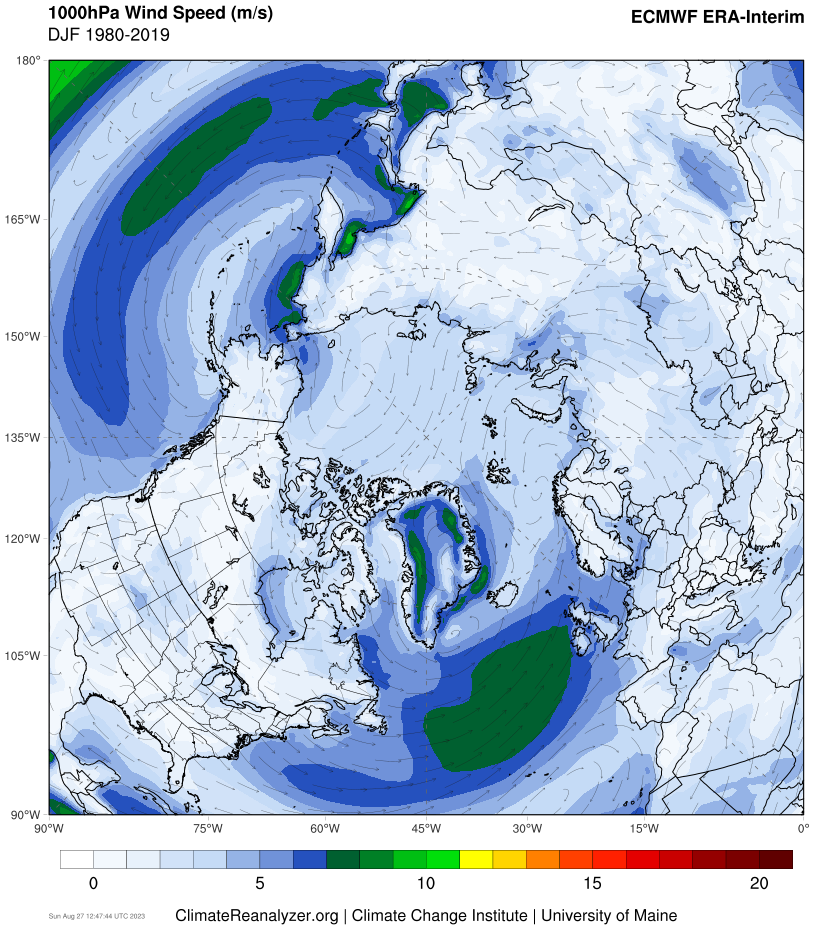
\includegraphics[width=\textwidth]{figures/erai_59.png}
        \caption{Sourced from \cite{ClimateReanalyzer2023}. 1000hPa average Wind Speed in m/s for the December-January-February period over the years 1980 to 2019. Based on ECMWF ERA-Interim reanalysis data. Easterly winds going into Europe display a meridonal curve. The wind speed over the mid-latitudes is greater when compared to the JJA period as presented in Figure \ref{fig:CR23_JJA_1000hPa_wind}.}
        \label{fig:CR23_DJF_1000hPa_wind}
    \end{figure}

    \begin{figure}
        \centering
        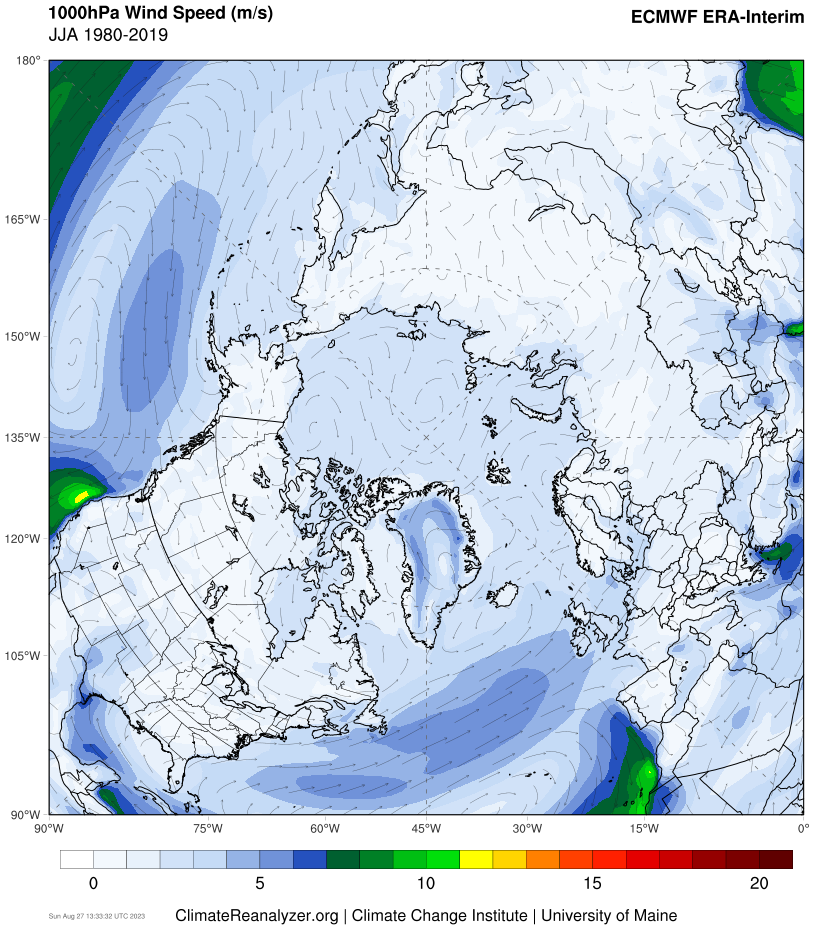
\includegraphics[width=\textwidth]{figures/erai_56.png}
        \caption{Sourced from \cite{ClimateReanalyzer2023}. 1000hPa average Wind Speed in m/s for the June-July-August period over the years 1980 to 2019. Based on ECMWF ERA-Interim reanalysis data. Easterly winds going into Europe follow a zonal trajectory.}
        \label{fig:CR23_JJA_1000hPa_wind}
    \end{figure}

\end{document}